\documentclass{beamer}
\usepackage{amsmath}
\usepackage[english]{babel} %set language; note: after changing this, you need to delete all auxiliary files to recompile
\usepackage[utf8]{inputenc} %define file encoding; latin1 is the other often used option
\usepackage{csquotes} % provides context sensitive quotation facilities
\usepackage{graphicx} %allows for inserting figures
\usepackage{booktabs} % for table formatting without vertical lines
\usepackage{textcomp} % allow for example using the Euro sign with \texteuro
\usepackage{stackengine}
\usepackage{wasysym}
\usepackage{tikzsymbols}
\usepackage{textcomp}
\newcommand{\bubblethis}[2]{
        \tikz[remember picture,baseline]{\node[anchor=base,inner sep=0,outer sep=0]%
        (#1) {\underline{#1}};\node[overlay,cloud callout,callout relative pointer={(0.2cm,-0.7cm)},%
        aspect=2.5,fill=yellow!90] at ($(#1.north)+(-0.5cm,1.6cm)$) {#2};}%
    }%
\tikzset{face/.style={shape=circle,minimum size=4ex,shading=radial,outer sep=0pt,
        inner color=white!50!yellow,outer color= yellow!70!orange}}
%% Some commands to make the code easier
\newcommand{\emoticon}[1][]{%
  \node[face,#1] (emoticon) {};
  %% The eyes are fixed.
  \draw[fill=white] (-1ex,0ex) ..controls (-0.5ex,0.2ex)and(0.5ex,0.2ex)..
        (1ex,0.0ex) ..controls ( 1.5ex,1.5ex)and( 0.2ex,1.7ex)..
        (0ex,0.4ex) ..controls (-0.2ex,1.7ex)and(-1.5ex,1.5ex)..
        (-1ex,0ex)--cycle;}
\newcommand{\pupils}{
  %% standard pupils
  \fill[shift={(0.5ex,0.5ex)},rotate=80] 
       (0,0) ellipse (0.3ex and 0.15ex);
  \fill[shift={(-0.5ex,0.5ex)},rotate=100] 
       (0,0) ellipse (0.3ex and 0.15ex);}

\newcommand{\emoticonname}[1]{
  \node[below=1ex of emoticon,font=\footnotesize,
        minimum width=4cm]{#1};}
\usepackage{scalerel}
\usetikzlibrary{positioning}
\usepackage{xcolor,amssymb}
\newcommand\dangersignb[1][2ex]{%
  \scaleto{\stackengine{0.3pt}{\scalebox{1.1}[.9]{%
  \color{red}$\blacktriangle$}}{\tiny\bfseries !}{O}{c}{F}{F}{L}}{#1}%
}
\newcommand\dangersignw[1][2ex]{%
  \scaleto{\stackengine{0.3pt}{\scalebox{1.1}[.9]{%
  \color{red}$\blacktriangle$}}{\color{white}\tiny\bfseries !}{O}{c}{F}{F}{L}}{#1}%
}
\usepackage{fontawesome} % Social Icons
\usepackage{epstopdf} % allow embedding eps-figures
\usepackage{tikz} % allows drawing figures
\usepackage{amsmath,amssymb,amsthm} %advanced math facilities
\usepackage{lmodern} %uses font that support italic and bold at the same time
\usepackage{hyperref}
\usepackage{tikz}
\hypersetup{
    colorlinks=true,
    linkcolor=blue,
    filecolor=magenta,      
    urlcolor=blue,
}
\usepackage{tcolorbox}
%add citation management using BibLaTeX
\usepackage[citestyle=authoryear-comp, %define style for citations
    bibstyle=authoryear-comp, %define style for bibliography
    maxbibnames=10, %maximum number of authors displayed in bibliography
    minbibnames=1, %minimum number of authors displayed in bibliography
    maxcitenames=3, %maximum number of authors displayed in citations before using et al.
    minnames=1, %maximum number of authors displayed in citations before using et al.
    datezeros=false, % do not print dates with leading zeros
    date=long, %use long formats for dates
    isbn=false,% show no ISBNs in bibliography (applies only if not a mandatory field)
    url=false,% show no urls in bibliography (applies only if not a mandatory field)
    doi=false, % show no dois in bibliography (applies only if not a mandatory field)
    eprint=false, %show no eprint-field in bibliography (applies only if not a mandatory field)
    backend=biber %use biber as the backend; backend=bibtex is less powerful, but easier to install
    ]{biblatex}
\addbibresource{../mybibfile.bib} %define bib-file located one folder higher


\usefonttheme[onlymath]{serif} %set math font to serif ones

\definecolor{beamerblue}{rgb}{0.2,0.2,0.7} %define beamerblue color for later use

%%% defines highlight command to set text blue
\newcommand{\highlight}[1]{{\color{blue}{#1}}}


%%%%%%% commands defining backup slides so that frame numbering is correct

\newcommand{\backupbegin}{
   \newcounter{framenumberappendix}
   \setcounter{framenumberappendix}{\value{framenumber}}
}
\newcommand{\backupend}{
   \addtocounter{framenumberappendix}{-\value{framenumber}}
   \addtocounter{framenumber}{\value{framenumberappendix}}
}

%%%% end of defining backup slides

%Specify figure caption, see also http://tex.stackexchange.com/questions/155738/caption-package-not-working-with-beamer
\setbeamertemplate{caption}{\insertcaption} %redefines caption to remove label "Figure".
%\setbeamerfont{caption}{size=\scriptsize,shape=\itshape,series=\bfseries} %sets figure  caption bold and italic and makes it smaller


\usetheme{Boadilla}

%set options of hyperref package
\hypersetup{
    bookmarksnumbered=true, %put section numbers in bookmarks
    naturalnames=true, %use LATEX-computed names for links
    citebordercolor={1 1 1}, %color of border around cites, here: white, i.e. invisible
    linkbordercolor={1 1 1}, %color of border around links, here: white, i.e. invisible
    colorlinks=true, %color links
    anchorcolor=black, %set color of anchors
    linkcolor=beamerblue, %set link color to beamer blue
    citecolor=blue, %set cite color to beamer blue
    pdfpagemode=UseThumbs, %set default mode of PDF display
    breaklinks=true, %break long links
    pdfstartpage=1 %start at first page
    }


% --------------------
% Overall information
% --------------------
\title[Principios de Economía]{Principios de Economía}
\date{}
\author[Ertola y Sturzenegger]{Gabriela Ertola y Federico Sturzenegger }
\vspace{0.4cm}
\institute[]{Universidad de San Andrés \\
2022} 


\begin{document}

\begin{frame}
\frametitle{Principios de Economía
\centering
\\ \vspace{12mm} Introducción a la Macroeconomía}
\centering
 \\ \vspace{12mm} %5 de agosto, 2021 \vspace{5mm} \\ 

\includegraphics[scale=0.25]{Figures/logoUDESA.jpg} 

\end{frame}


\begin{frame}
\frametitle{La micro y la macro}
\begin{itemize}
        \item Disciplinas dentro de economía
        \vspace{2mm}
        \begin{itemize}
        \item Hasta ahora hemos visto cosas que se suelen asociar con la microeconomía \\
        - ¿Cómo los agentes interactúan entre sí y toman decisiones?
        \vspace{2mm}
        \item Ahora nos metemos en temas de macroeconómica \\
        - ¿Cómo funciona la economía en su conjunto, donde cambios económicos afectan a los agentes en forma simultánea?
        \end{itemize}
\end{itemize}
\end{frame}


\begin{frame}{Macroeconomía}
   \begin{itemize}
       \item La macroeconomía tiene que ver con los resultados "agregados" de la economía \vspace{1mm}
       \item Vamos a ver qué son y cómo medir los agregados económicos: la actividad, los precios, el desempleo, etc. \vspace{1mm}
       \item También vamos a estudiar los ciclos económicos: porque el crecimiento viene acompañado de booms y recesiones \vspace{1mm}
       \item Finalmente, vamos a discutir políticas: ¿qué variables afectan la política fiscal y monetaria? 
   \end{itemize} 
\end{frame}

\begin{frame}
\frametitle{ Evaluando toda la economía}
\begin{itemize}
        \item Para evaluar la forma en que una persona está en términos económicos uno suele mirar sus ingresos \vspace{1mm}
        \item Para una economía hacemos lo mismo, pero una economía es un sistema en el que diversos agentes interactúan \vspace{1mm}
        \begin{itemize}
            \item Hogares
            \item Empresas
            \item Instituciones financieras
            \item Gobierno
            \item Sector externo
        \end{itemize}
\end{itemize}
\end{frame}

\begin{frame}{Flujo circular de la riqueza}
    \begin{figure} [H]
\centering
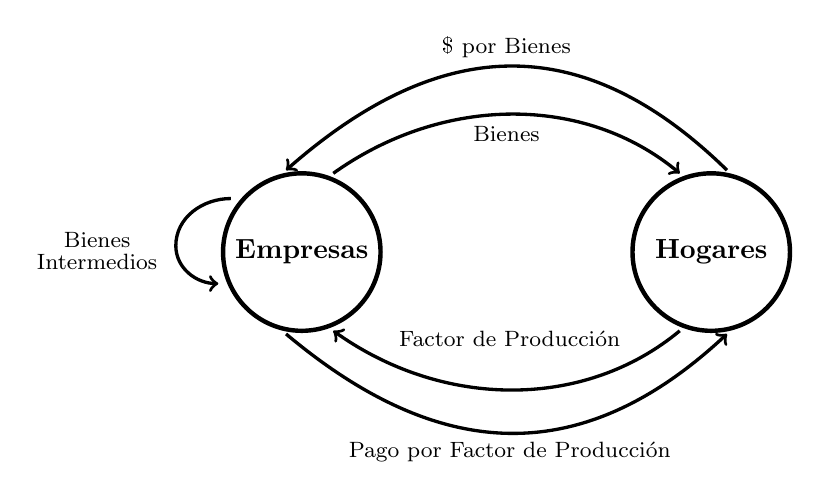
\begin{tikzpicture}[scale=0.4]
\draw[ultra thick](2,0) circle [radius =2.5];
\node[] at (2,0) { \textbf{Empresas}};
\draw[ultra thick](15,0) circle [radius =2.5];
\node[] at (15,0) {\textbf{Hogares} };
\draw [very thick, ->] (-0.25, 1.7) to [out=-180, in=90] (-2, 0.2) to [out=-90, in=180] (-0.65, -1);
\node[] at (-4.5,0.4) {\footnotesize  Bienes};
\node[] at (-4.5,-0.3) {\footnotesize  Intermedios};
\draw[very thick, ->] (3,2.5).. controls (6.5,5) and (11,5) .. (14,2.5);
\draw[very thick, <-] (1.5,2.6).. controls (6.5,7) and (11,7) .. (15.5,2.6);
\node[] at (8.5,3.75) {\footnotesize  Bienes};
\node[] at (8.5,6.5) {\footnotesize  \$ por Bienes};
\draw[very thick, <-] (3,-2.5).. controls (6.5,-5) and (11,-5) .. (14,-2.5);
\draw[very thick, ->] (1.5,-2.6).. controls (6.5,-6.8) and (11,-6.8) .. (15.5,-2.6);
\node[] at (8.6,-2.75) {\footnotesize  Factor de Producción};
\node[] at (8.6,-6.35) {\footnotesize Pago por Factor de Producción};
\end{tikzpicture}
\label{fig:25.1}
\end{figure} 

\end{frame}


\begin{frame}{Definiendo el PBI}
\begin{itemize}
   \item El Producto Bruto Interno (PBI) es una medida del producto total de una economía \vspace{1mm}
   \item ¡Noten que la suma de los bienes es igual a la suma de los ingresos! \vspace{1mm}
   \item Por eso a veces nos referimos al PBI como ingreso nacional
   \end{itemize}
\end{frame}

\begin{frame}
\frametitle{ El PBI}
\begin{itemize}
        \item Mirándolo en términos de gasto, el PBI es el valor de mercado de todos bienes finales y servicios producidos en una economía durante un período de tiempo determinado \vspace{1mm}
        \begin{itemize}
            \item ``Valor de mercado'' \\ 
            - Utiliza los precios que la gente está dispuesta a pagar \vspace{1mm}
            \item ``todos los bienes finales y servicios'' \\
            - Bienes tangibles y servicios intangibles \\
            - No se cuenta bienes intermedios \\
            - Todo lo producido en la economía, vendido legalmente \\ \vspace{1mm}
            \item ``en una economía, durante un período determinado'' \\
            - Producción dentro de los límites geográficos \\
            - Un flujo de un intervalo de tiempo \\ 
        \end{itemize}
\end{itemize}
\end{frame}


\begin{frame}{ Midiendo el PBI}
    \begin{itemize}
        \item Tenemos tres maneras de medirlo \vspace{1mm}
       \begin{itemize}
           \item Por el gasto (valor de los bienes finales consumidos) \vspace{1mm}
           \item Por los ingresos (suma de los ingresos recibidos) \vspace{1mm}
           \item La producción (total producido por la industria) \\
            - Aquí se mide el valor agregado en la producción de cada industria
       \end{itemize}
    \end{itemize}
\end{frame}

\begin{frame}{Un ejemplo de cómo medir el PBI}
    \begin{figure} [H]   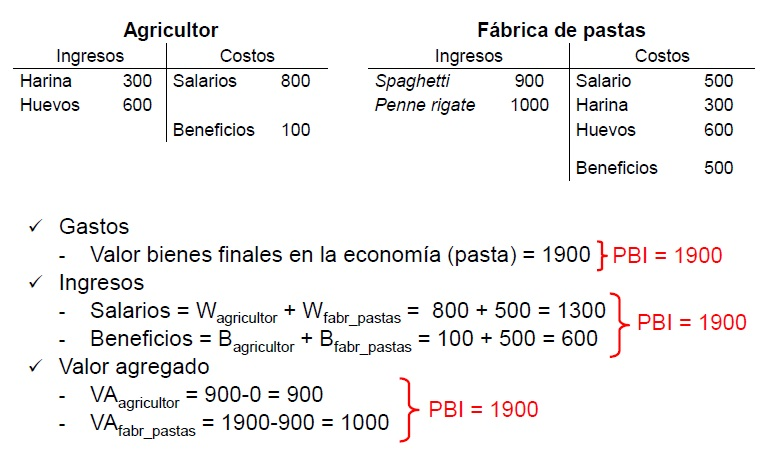
\includegraphics[scale=0.55]{Figures/C16.2.jpg}
\label{fig:25.2}
\end{figure}

\end{frame}

\begin{frame}{Buscando los datos}
    \begin{itemize}
        \item Cada país tiene su agencia de estadísticas \vspace{1mm}
        \item En Argentina es el Indec \vspace{1mm}
        \item Pueden ver también Alphacast \vspace{1mm}
        \item Para bases de datos homogéneas: IFS \vspace{1mm}
        \item Para perspectivas futuras: WEO \vspace{1mm}
        \item Para otra visión: FRED
        
    \end{itemize}
\end{frame}

\begin{frame}
\frametitle{ Otros elementos importantes}
\begin{itemize}
        \item ¿Cómo incorporamos el sector externo?
        \begin{itemize}
            \item Parte de la producción extranjera es el consumo interno (importaciones) y parte de la producción nacional es consumo extranjero (exportaciones) \\ 
            - El PBI incluye valor agregado, ingresos de, o consumo de producción nacional \\
            - Incluimos exportaciones y excluimos importaciones
            \end{itemize} \vspace{1mm}
        \item ¿Cómo incorporamos al gobierno?
        \begin{itemize}
            \item Se lo trata básicamente como otro productor \\
            - Servicios públicos son “comprados” con impuestos \\
            - El costo de producción captura la valor agregado
            \end{itemize}
\end{itemize}
\end{frame}


\begin{frame}{PBI y PBN}
    \begin{itemize}
        \item El Producto Bruto Nacional (PBN) es el PBI ajustado por el retorno a los factores externos
    \end{itemize}
    \begin{table}
    \small
\begin{tabular}{|c|c|c|c|} 
\hline 
\multicolumn{2}{|c|}{\textbf{Top PBI}} & \multicolumn{2}{c|}{\textbf{Top PNB}} \\ \hline
1. Luxembourg              & 116.921   & 1.  Macao                  & 116.080  \\ \hline
2.  Switzerland            & 86.849    & 2. Qatar                   & 91.499   \\ \hline
\textbf{3. Ireland}        & 83.849    & 3.  Singapore              & 87.735   \\ \hline
4. Norway                  & 67.176    & 4. Bermuda                 & 85.191   \\ \hline
5. United States           & 63.415    & 5. Luxembourg              & 72.145   \\ \hline
6. Brunei Darussalam       & 59.123    & 6. Switzerland             & 68.992   \\ \hline
7. Hong kong               & 56.420    & 7.  United Arab Emirates   & 67.462   \\ \hline
8. Denmark                 & 55.864    & 8. Norway                  & 66.749   \\ \hline
9. United Arab Emirates    & 55.693    & \textbf{9. Ireland}        & 66.668   \\ \hline
10. San Marino             & 55.384    & 10. Brunei Darussalam      & 63.963   \\ \hline
\end{tabular}
\end{table}
\end{frame}

\begin{frame}{Un caso extraordinario }
    
\begin{figure} [H]
\centering
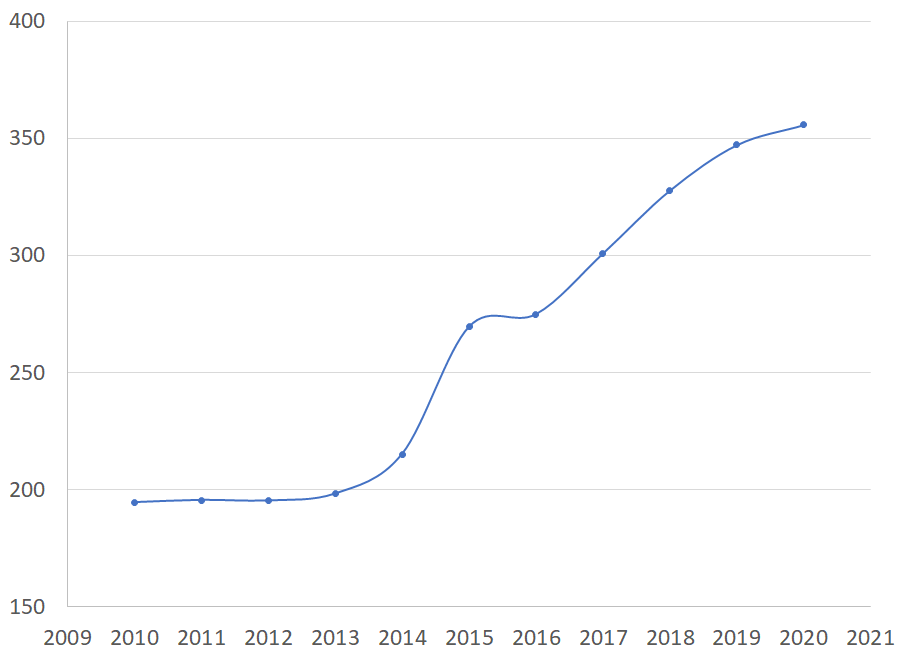
\includegraphics[]{Figures/G1.png}
\caption{PBI Irlanda a precios constantes}
\label{fig:G1}
\end{figure} 
\end{frame}

\begin{frame}{Temas en la medición del PBI}
    \begin{itemize}
        \item Ventas de bienes ya producidos no van (ejemplo: venta de una casa)
        \item Transferencias de ingresos no van (ejemplo: jubilaciones) 
        \item ¿Planes sociales? Depende! (ejemplo: AUH vs Plan Jefes y Jefas de Hogares)
        \item Se incorpora una estimación de la economía informal
        \item Los bienes y servicios producidos por el Estado tambien deben incorporarse
        \begin{itemize}
            \item Pero al ser difícil asignar un valor de mercado a estos bienes y servicios, se los agrega al costo de producción
        \end{itemize}
        \item Algunas discusiones: productos de internet y ajustes por calidad
    \end{itemize}
\end{frame}


\begin{frame}{Graficando el PBI de EEUU a largo plazo}
    \begin{figure} [H]   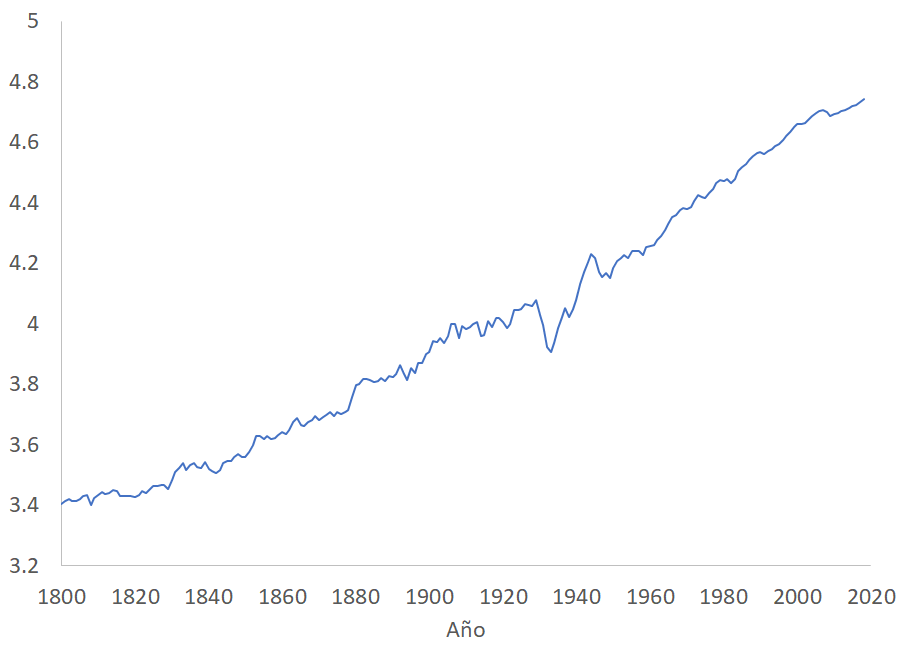
\includegraphics[scale=1]{Figures/G2.png}
\end{figure}
\end{frame}

\begin{frame}{Ajustando con logs}
    \begin{center}
\begin{figure}[H]
\renewcommand{\figurename}{Figure}
\begin{center}
    \begin{minipage}[b]{0.35\textwidth}
        \begin{center}
\begin{tikzpicture}[scale=0.4]
\draw[very thick,<->] (0,11) node[left]{$f$}--(0,0)--(11,0) node[below]{$x$};
\draw[semithick] (0,1).. controls (3,1) and (8, 1.1) .. (8.5, 8) node [right]{\footnotesize $Ae^{\lambda x}$};
\end{tikzpicture}
\end{center}
     \end{minipage}
  %  \hfill
    \begin{minipage}[b]{0.4\textwidth}
    \begin{center}
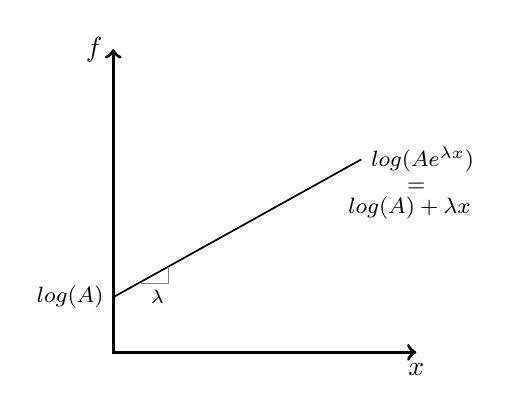
\begin{tikzpicture}[scale=0.35]
\draw[very thick,<->] (0,11) node[left]{$f$}--(0,0)--(11,0) node[below]{$x$};
\draw[semithick] (0,2)--(9, 7) node [right]{\footnotesize $log(Ae^{\lambda x})$};
\draw[semithick, gray] (1,2.5)--(2,2.5)--(2,3.1);
\node[] at (1.6,2) {\scriptsize $\lambda$};
\node[left] at (0,2) {\footnotesize $log(A)$};
\node[] at (11,6) {\footnotesize $=$};
\node[] at (10.75,5.25) {\footnotesize $log(A)+\lambda x$};
\end{tikzpicture}
\end{center}
    \end{minipage}
\end{center}
\end{figure}
\end{center} 
\end{frame}

\begin{frame}{Re-graficando el PBI de EEUU a largo plazo en logs}
   \begin{figure} [H]   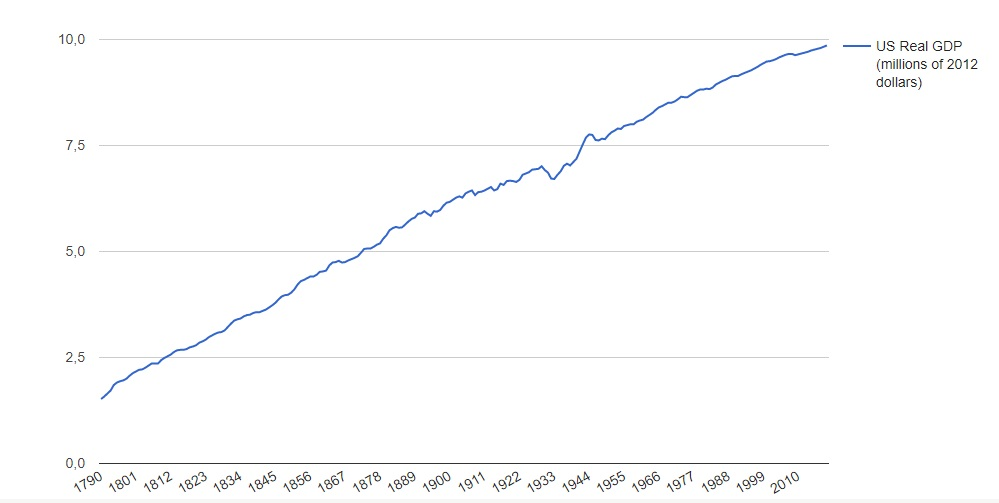
\includegraphics[scale=0.45]{Figures/C16.4.jpg}
\end{figure}
Fuente: \href{https://www.measuringworth.com/graphs/}{www.measuringworth.com}
\end{frame}

\begin{frame}
\frametitle{Argentina y el crecimiento mundial}
\begin{center}
\href{https://www.gapminder.org/tools/#$model$markers$line$data$filter$dimensions$country$country$/$in@=usa&=chn&=arg&=bra&=nzl&=can&=aus;;;;;;&encoding$selected$data$filter$markers@=aus&=arg;;;;;;;;&chart-type=linechart&url=v1} {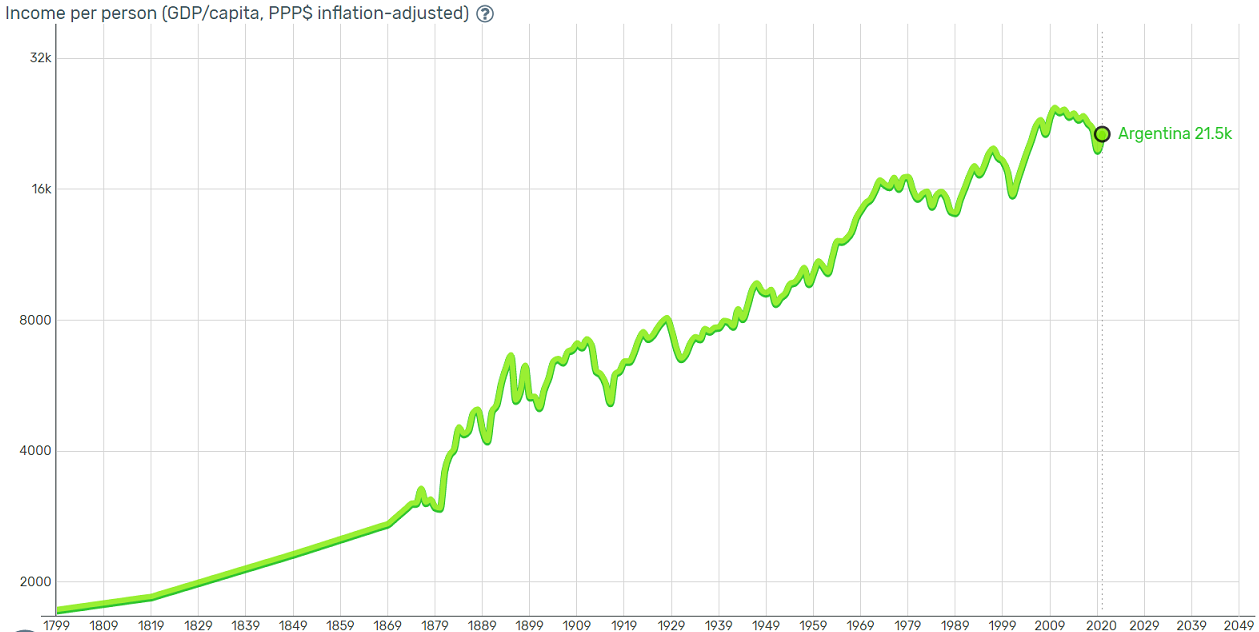
\includegraphics[width=0.9\textwidth]{Figures/gdparg.png}}
\end{center}
Fuente: Gapminder
\end{frame}

\begin{frame}
\frametitle{PBI real y nominal}
\begin{itemize}
        \item Pensemos en la definición del PBI nominal
        \\ \vspace{1mm}
        \begin{center} \small{
            $PBI_{nominal}^{\text{año t}}=p_{1}^{\text{año t}}q_{1}^{\text{año t}}+p_{2}^{\text{año t}}q_{2}^{\text{año t}}+...+p_{N}^{\text{año t}}q_{N}^{\text{año t}}$}
        \end{center}
        \\ \vspace{1mm}
        \begin{itemize}
            \item Si el gasto se eleva de un año al siguiente: \\
            - ¿Se está produciendo más en la economía? \\
            - ¿Los bienes y servicios se venden a precios más altos?
            \end{itemize} \vspace{1mm}
        \item El PBI real
        \begin{itemize}
            \item ¿Cuál sería el valor de los bienes y servicios producidos en un año si los valoramos a precios que prevalecieron en algún año específico? \\
            - ¿Qué es una buen año ‘base’?
            \end{itemize} \vspace{1mm}
        \item ¿Por qué es importante la diferencia entre nominal y real? \href{https://www.gapminder.org/tools/#$model$markers$line$data$filter$dimensions$country$country$/$in@=arg;;;;;;&encoding$y$data$concept=inflation_annual_percent&space@=country&=time;;&scale$type:null&domain:null&zoomed:null;;&frame$value=2013;;;;;&chart-type=linechart&url=v1}{Exploremos}
\end{itemize}
\end{frame}

\begin{frame}
\frametitle{PBI real vs. nominal}
\begin{itemize}
        \item PBI nominal (a precios corrientes) 
         \\ \vspace{1mm}
        \begin{center} \small{
            $PBI_{nominal}^{\text{año i}}=p_{1}^{\text{año i}}q_{1}^{\text{año i}}+p_{2}^{\text{año i}}q_{2}^{\text{año i}}+...+p_{N}^{\text{año i}}q_{N}^{\text{año i}}$}
            \\ \vspace{1mm}
            \small{
            $PBI_{nominal}^{\text{año j}}=p_{1}^{\text{año j}}q_{1}^{\text{año j}}+p_{2}^{\text{año j}}q_{2}^{\text{año j}}+...+p_{N}^{\text{año j}}q_{N}^{\text{año j}}$}
        \end{center}
         \\ \vspace{1mm}
        \item PBI real (a precios constantes) 
         \\ \vspace{1mm}
         \begin{center} \small{
            $PBI_{real}^{\text{año i}}=p_{1}^{\text{año b}}q_{1}^{\text{año i}}+p_{2}^{\text{año b}}q_{2}^{\text{año i}}+...+p_{N}^{\text{año b}}q_{N}^{\text{año i}}$}
            \\ \vspace{1mm}
            \small{
            $PBI_{real}^{\text{año j}}=p_{1}^{\text{año b}}q_{1}^{\text{año j}}+p_{2}^{\text{año b}}q_{2}^{\text{año j}}+...+p_{N}^{\text{año b}}q_{N}^{\text{año j}}$}
        \end{center}
        
\end{itemize}
\end{frame}


\begin{frame}{PBI nominal y real de EEUU}
    \begin{figure} [H]   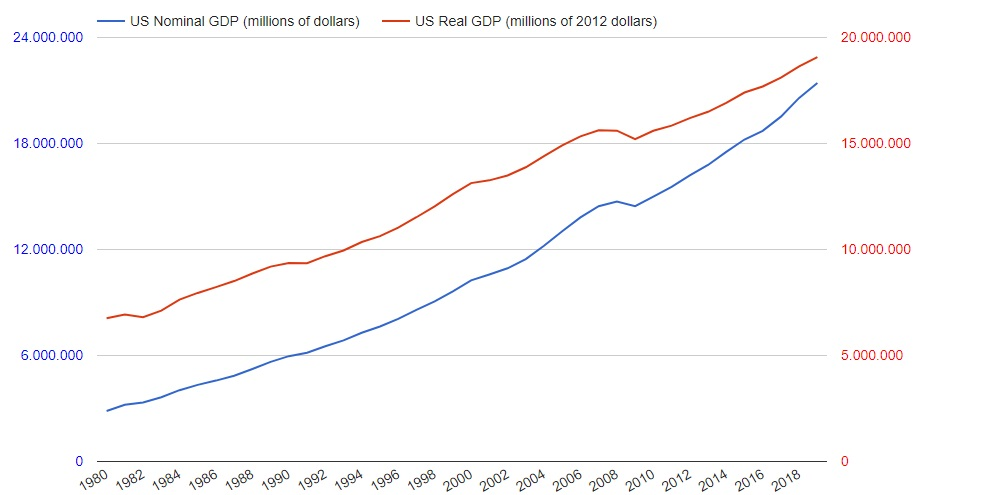
\includegraphics[scale=0.4]{images/C16.5.jpg}
\label{fig:25.5}
\end{figure}
Fuente: \href{https://www.measuringworth.com/graphs/}{www.measuringworth.com}
\end{frame}
 

\begin{frame}{PBI Nominal y real de Argentina}
    \begin{figure} [H]   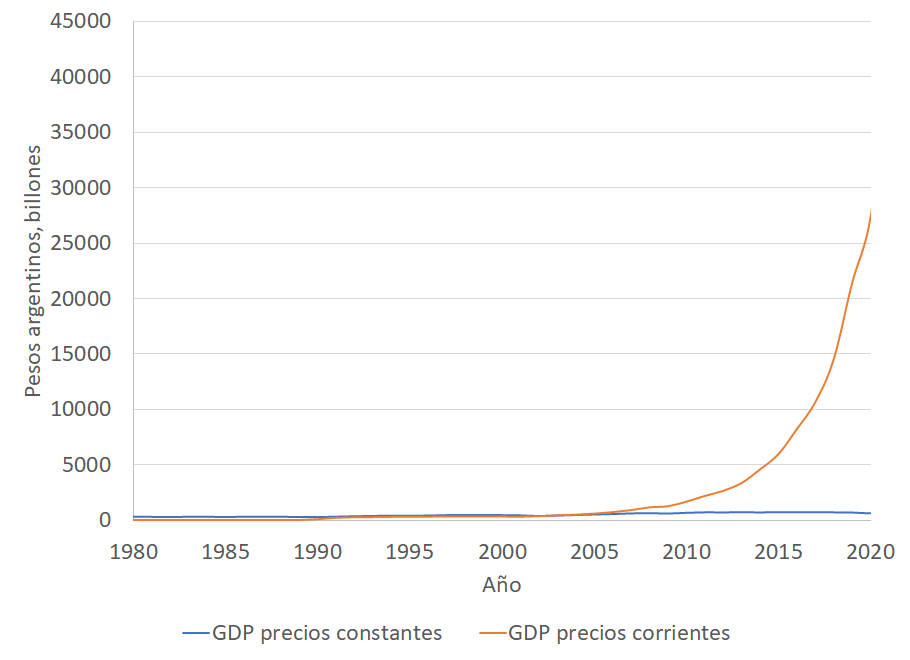
\includegraphics[scale=1.1]{Figures/G2B.png}
\end{figure}
\end{frame}


\begin{frame}{Componentes y desglose del PBI}
    \begin{itemize}
    \item Haciendo referencia a los sectores que los producen (se originan en la agricultura, la minería, la industria, el comercio, el turismo, etc.) 
        \begin{itemize} \vspace{1mm}
            \item A esta referencia la llamaremos el \textit{PBI por el lado de la oferta}
        \end{itemize} \vspace{2mm}
     \item Según el uso de los bienes: vamos a segmentar el PBI según los bienes se usan para el consumo, la  inversión, el consumo público, el sector externo o la acumulación de inventarios \vspace{1mm}
     \begin{itemize}
            \item A esto lo llamaremos el \textit{PBI por el lado de la demanda}
        \end{itemize}
\end{itemize}
\end{frame}

\begin{frame}{El PBI por el lado de la oferta}
    \begin{table}[H] 
\resizebox{.62\textwidth}{!}{%
\begin{tabular}{|c|c|}
\hline
\textbf{Elementos del PBI - Oferta}                                                                               & \textbf{Millones de pesos corrientes} \\ \hline
\begin{tabular}[c]{@{}c@{}}A - Agricultura, ganadería, caza \\ y silvicultura\end{tabular}                        & 1.543.784                             \\ \hline
B - Pesca                                                                                                         & 86.525                                \\ \hline
\begin{tabular}[c]{@{}c@{}}C - Explotación de minas \\ y canteras\end{tabular}                                    & 857.865                               \\ \hline
D - Industria manufacturera                                                                                       & 4.223.679                             \\ \hline
E - Electricidad, gas y agua                                                                                      & 438.732                               \\ \hline
F - Construcción                                                                                                  & 885.981                               \\ \hline
\begin{tabular}[c]{@{}c@{}}G - Comercio mayorista, minorista \\ y reparaciones\end{tabular}                       & 4.451.862                             \\ \hline
H - Hoteles y restaurantes                                                                                        & 312.971                               \\ \hline
\begin{tabular}[c]{@{}c@{}}I - Transporte, almacenamiento \\ y comunicaciones\end{tabular}                        & 1.320.842                             \\ \hline
J - Intermediación financiera                                                                                     & 999.990                               \\ \hline
\begin{tabular}[c]{@{}c@{}}K - Actividades inmobiliarias, \\ empresariales y de alquiler\end{tabular}             & 2.655.948                             \\ \hline
L - Administración pública y defensa                                                                              & 1.890.537                             \\ \hline
M - Enseñanza                                                                                                     & 1.457.592                             \\ \hline
N - Servicios sociales y de salud                                                                                 & 1.237.435                             \\ \hline
\begin{tabular}[c]{@{}c@{}}O - Otras actividades de servicios \\ comunitarias, sociales y personales\end{tabular} & 524.134                               \\ \hline
\begin{tabular}[c]{@{}c@{}}P - Hogares privados con servicio \\ doméstico\end{tabular}                            & 157.032                               \\ \hline
\end{tabular}%
}
\caption{PBI Argentina 2020 - Oferta}
\label{Tab:T38.3}
\end{table}
\end{frame}

\begin{frame}{El PBI por el lado de la demanda}
    \begin{table}[H]
\begin{tabular}{|c|c|}
\hline
\textbf{Elementos del PBI - Demanda} & \textbf{Millones de pesos corrientes} \\ \hline
Consumo privado                      & 17.456.121                            \\ \hline
Consumo publico                      & 4.268.255                             \\ \hline
Exportaciones                        & 4.559.670                             \\ \hline
Importaciones                        & 3.725.473                             \\ \hline
Formación bruta de capital fijo      & 3.816.717                             \\ \hline
\end{tabular}
\caption{PBI Argentina 2020 - Demanda}
\label{Tab:T38.2}
\end{table}

\end{frame}



\begin{frame}{El PBI por la demanda}
    
  \begin{equation}
        Y= C + I + G + X - M +  \Delta Inv.
  \end{equation}
  \begin{itemize}
  \item Esta es una ecuación muy conocida en macroeconomía
  \end{itemize}
\end{frame}

\begin{frame}{¿Cómo se compara el PBI entre países?}
    \begin{figure} [H]   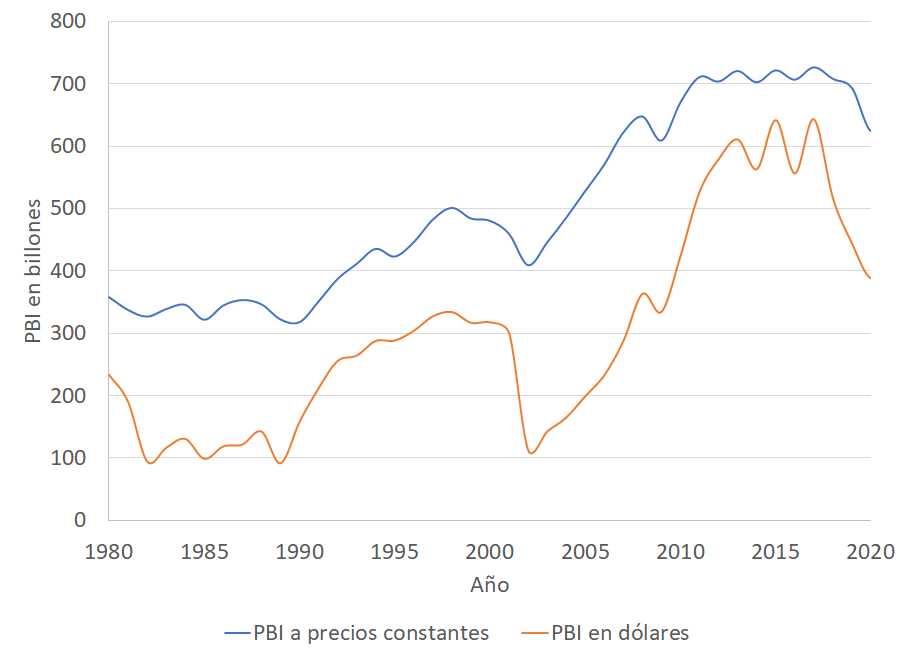
\includegraphics[scale=1.04]{Figures/G3.png}
\end{figure}
\end{frame}
                   
\begin{frame}{PBI en dólares y PBI en PPP}
\begin{itemize}
    \item PBI de EEUU es USD 59.041 \vspace{1mm}
    \item PBI de India es 142.073 rupias \vspace{1mm}
    \item PBI de India (en USD) es de USD 965  \vspace{1mm}
    \item Una mejor medida es el PBI de India medido en los precios de EEUU \vspace{1mm}
    \item Con ese cálculo el PBI PPP de India es de 6.461
\end{itemize}
\end{frame}

\begin{frame}{Una comparación India-China-EEUU}
   \begin{figure}[H]
\centering
    \subfigure{
\resizebox{0.42\textwidth}{!}{%
    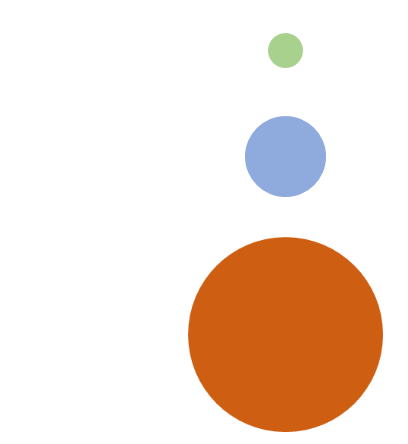
\includegraphics[width=0.9\textwidth]{Figures/G4.2A.png}}}
  \hfill 
    \subfigure{
\resizebox{0.42\textwidth}{!}{%
    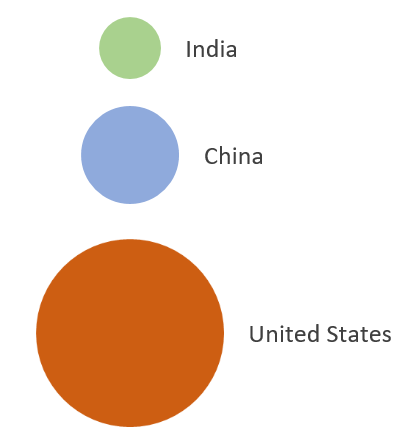
\includegraphics[width=0.9\textwidth]{Figures/G4.2B.png}}}
\end{figure} 
\end{frame}

\begin{frame}{Otra comparación}
    \begin{figure} [H]   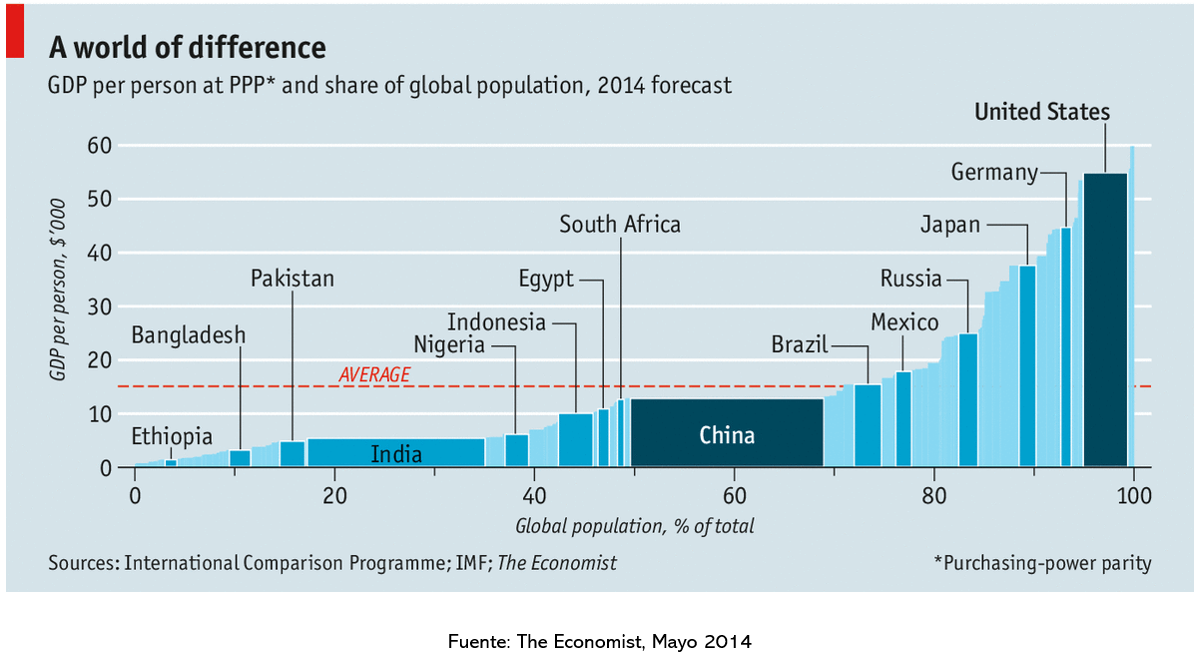
\includegraphics[scale=0.4]{Figures/C16.6.png}
\caption{\textbf{¿Cómo comparamos los ingresos en el mundo?}}
\label{fig:16.6}
\end{figure}

\end{frame}


\begin{frame}{Índice de desarrollo humano}
    Las Naciones Unidas (ONU) crearon el Índice de Desarrollo Humano que está conformado por tres indicadores claves: \vspace{1mm}
\begin{itemize}
    \item Ingresos (PBI per cápita ajustado por PPP) \vspace{1mm}
    \item Longevidad (esperanza de vida al nacer) \vspace{1mm}
    \item Conocimiento (alfabetización y años de estudio).
\end{itemize} \vspace{2mm}
    Es un indicador mas amplio del bienestar que el estrictamente económico

\end{frame}


\begin{frame}{Índice de desarrollo humano 2019}
\begin{figure} [H]  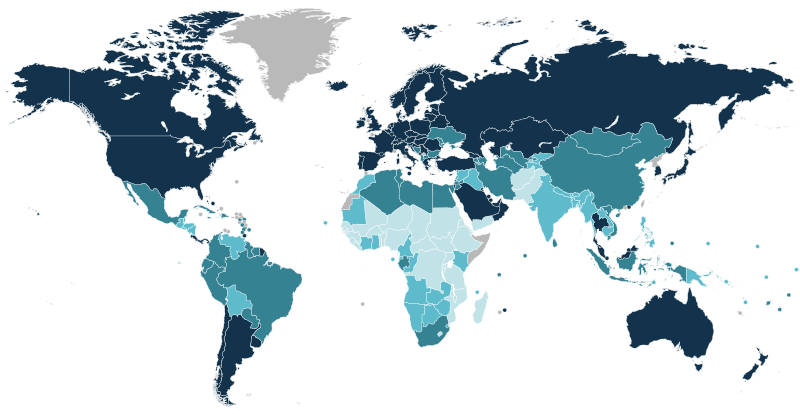
\includegraphics[scale=0.4]{Figures/C16.7.png}
\end{figure}
\end{frame}


\begin{frame}{Midiendo la inflación}
\begin{itemize}    
    \item Típicamente para medir la inflación se elige una canasta de bienes \vspace{1mm}
    \item Definida la canasta de bienes, el nivel de precios es: 
        \begin{equation}
            P_t = p_1 q_1^c+ p_2 q_2^c...p_n q_n^c,
        \end{equation}

    \\ donde $q_i^c$ es la participación del bien $i$ en la canasta de consumo que se considera

    \item A su vez la tasa de inflación sería 

    \begin{equation}
        \pi =\frac{P_t - P_{t-1}}{P_{t-1}}= \frac{\vartriangle P}{P_{t-1}}.
    \end{equation}
\end{itemize}
\end{frame}

\begin{frame}{Problemas con el índice}
    \begin{itemize}
        \item Eligiendo la canasta \vspace{1mm}
        \item Ajustando por calidad \vspace{1mm}
        \item Sesgo de sustitución \vspace{1mm}
        \item Sesgo de sub-reporte \vspace{1mm}
        \item Hay distintos tipos de índices de precios (consumidor, construcción, etc.)
    \end{itemize}
\end{frame}

\begin{frame}{Deflactor del PBI }
\begin{itemize}
\item ¿Existe una medida de precios del conjunto de bienes de la economía? \\ \vspace{2mm}
El deflactor del PBI es
        \begin{center}                              $PBI_{deflactor}^{\text{año i}}=\frac{PBI_{nominal}^{\text{año i}}}{PBI_{real}^{\text{año i}}} x 100$
        \end{center}
\end{itemize}
\end{frame}


\begin{frame}
\frametitle{Tomemos una economía}
\begin{center}
    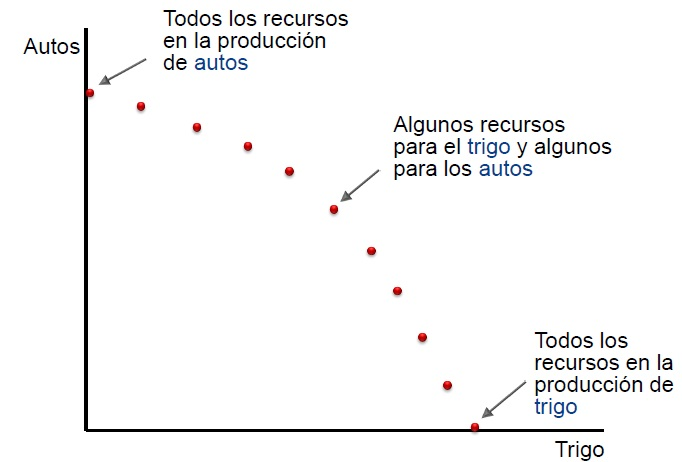
\includegraphics[scale=0.6]{Tema_11.2_tomemosunaeconomia.jpg}
\end{center}
\end{frame}

\begin{frame}
\frametitle{Frontera de posibilidades}
\begin{center}
    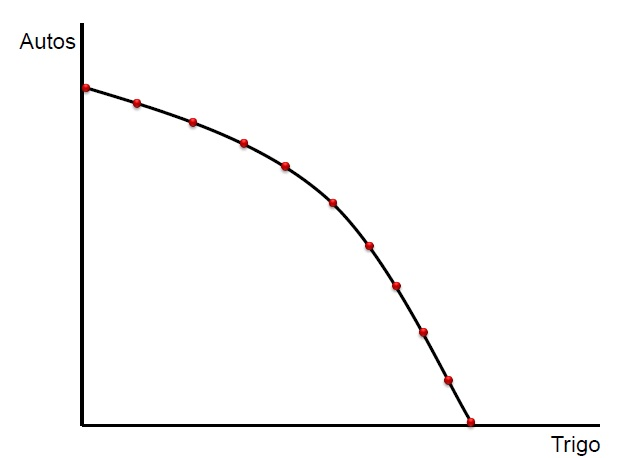
\includegraphics[scale=0.6]{Tema_11.3_frontera.jpg}
\end{center}
\end{frame}

\begin{frame}
\frametitle{Frontera de posibilidades}
\begin{center}
    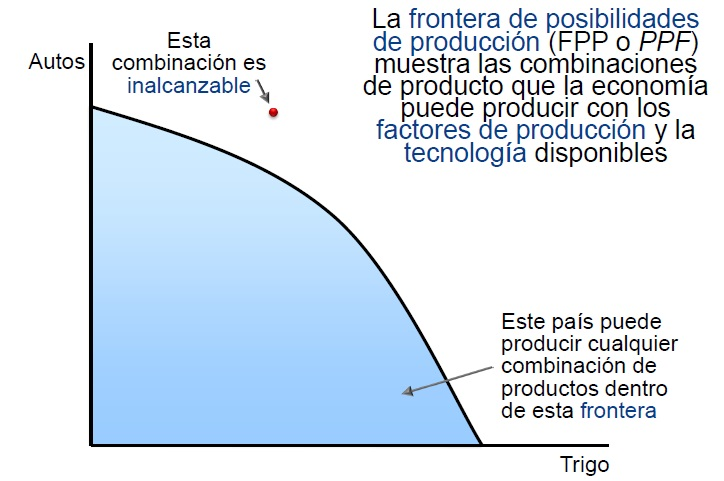
\includegraphics[scale=0.55]{Tema_11.4_fronteradeposibilidades.jpg}
\end{center}
\end{frame}

\begin{frame}
\frametitle{Fuera de la frontera}
\begin{center}
    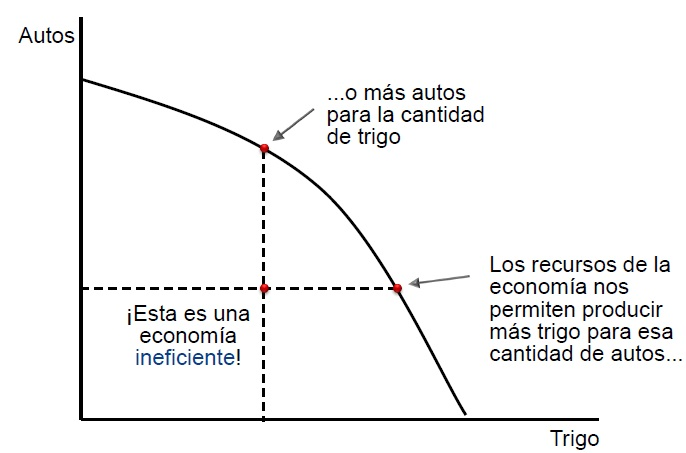
\includegraphics[scale=0.6]{Tema_11.5_fueradelafrontera.jpg}
\end{center}
\end{frame}

\begin{frame}
\frametitle{Misma frontera}
\begin{center}
    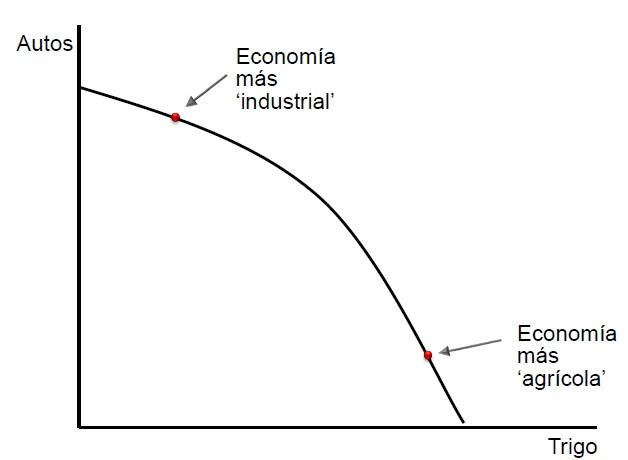
\includegraphics[scale=0.6]{Tema_11.6_lamismafrontera.jpg}
\end{center}
\end{frame}

\begin{frame}
\frametitle{Cambio en la tecnología}
\begin{center}
    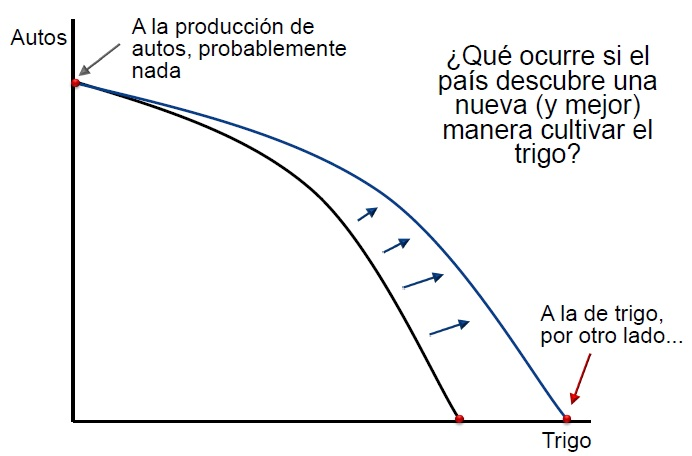
\includegraphics[scale=0.6]{Tema_11.7_cambiotecnologico.jpg}
\end{center}
\end{frame}

\begin{frame}
\frametitle{Cambio en los factores}
\begin{center}
    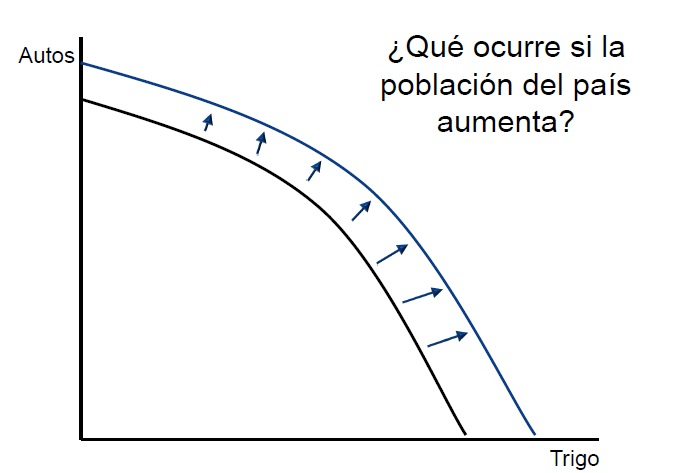
\includegraphics[scale=0.55]{Tema_11.8_cambioenlosfactores.jpg}
\end{center}
\end{frame}

\begin{frame}
\frametitle{ Shock exógeno}
\begin{center}
    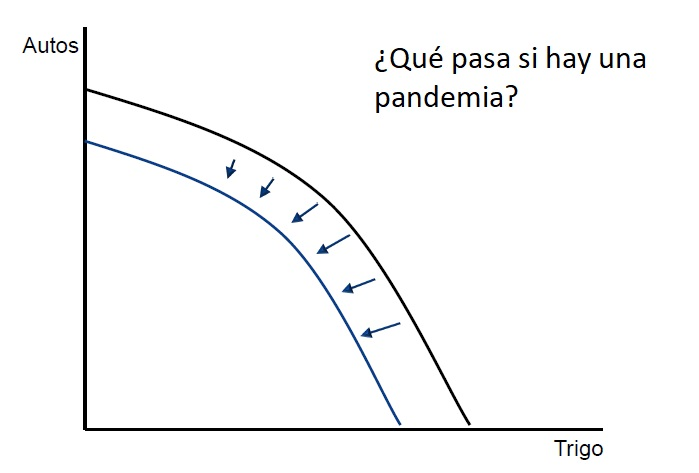
\includegraphics[scale=0.6]{Tema_11.9_pandemia.jpg}
\end{center}
\end{frame}

\begin{frame}
\frametitle{ Cambios en el equilibrio}
\begin{center}
    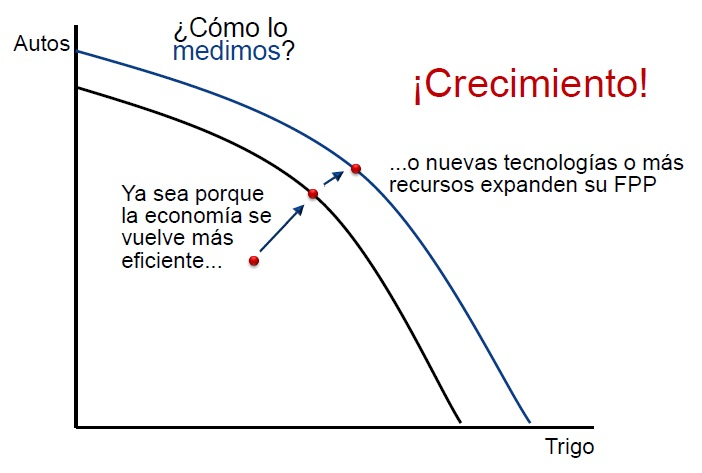
\includegraphics[scale=0.6]{Tema_11.10_crecimiento.jpg}
\end{center}
\end{frame}

\begin{frame}
\frametitle{ Luces nocturnas}
\begin{center}
    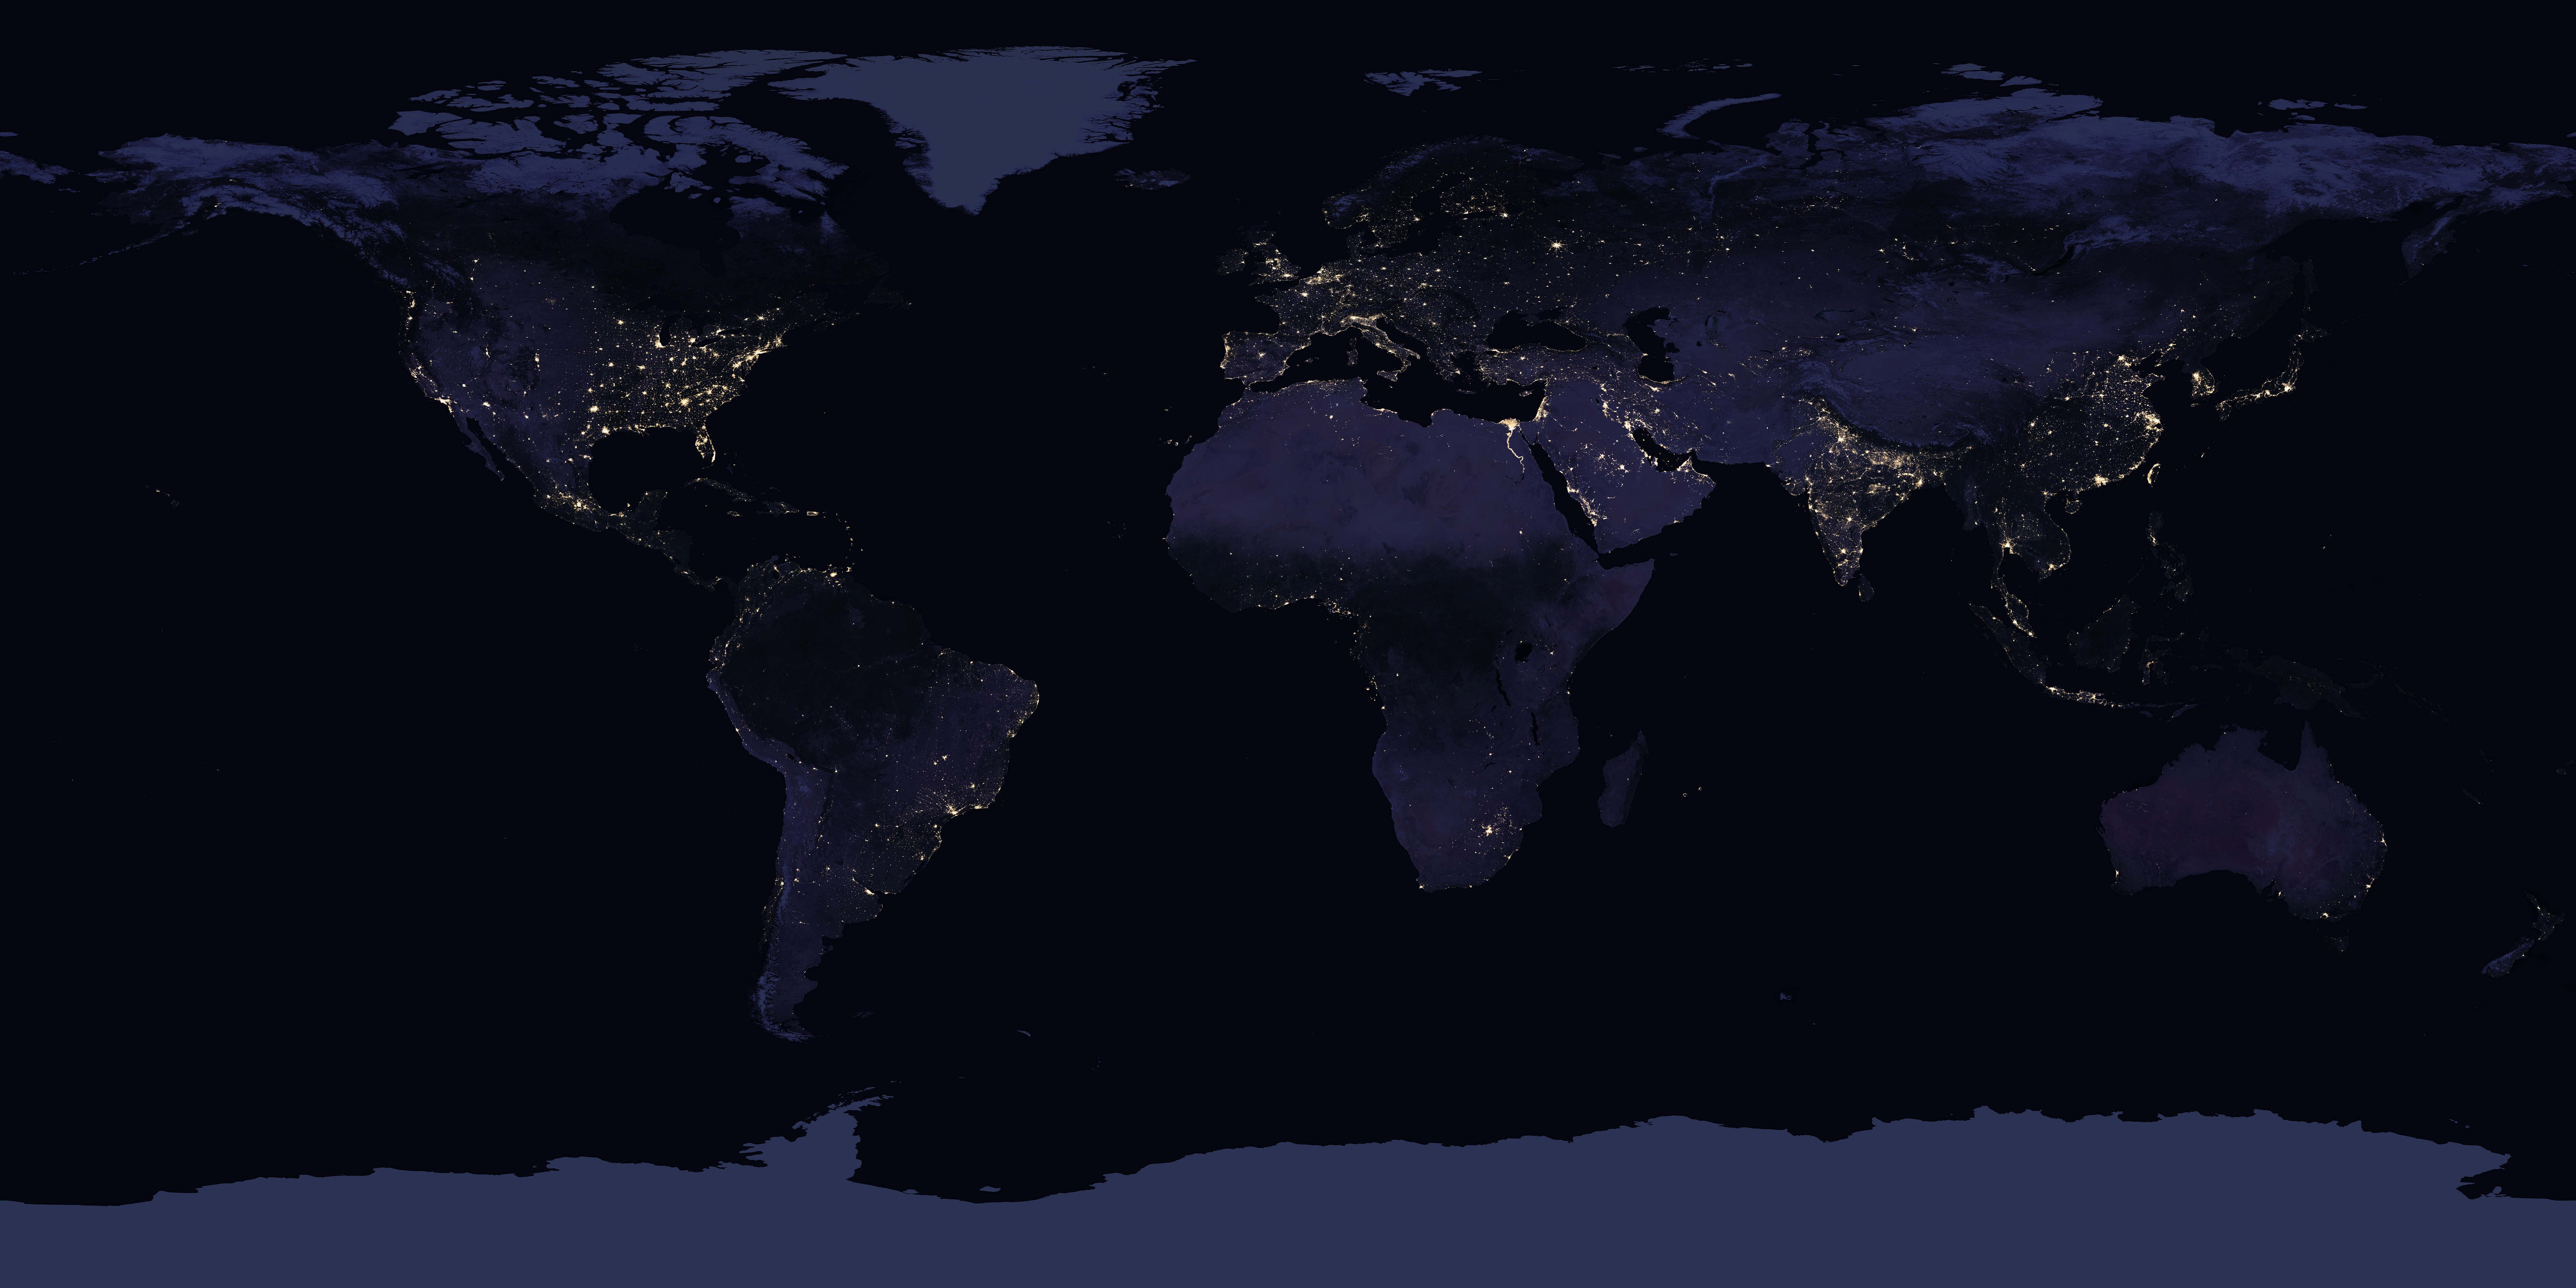
\includegraphics[scale=0.06]{Tema_11.11_crecimiento2.jpg}
\end{center}
Fuente: \href{https://www.nasa.gov/feature/goddard/2017/new-night-lights-maps-open-up-possible-real-time-applications}{NASA}
\end{frame}

\begin{frame}
\frametitle{Crecimiento}
\begin{center}
    \href{https://ourworldindata.org/grapher/gdp-per-capita-worldbank} {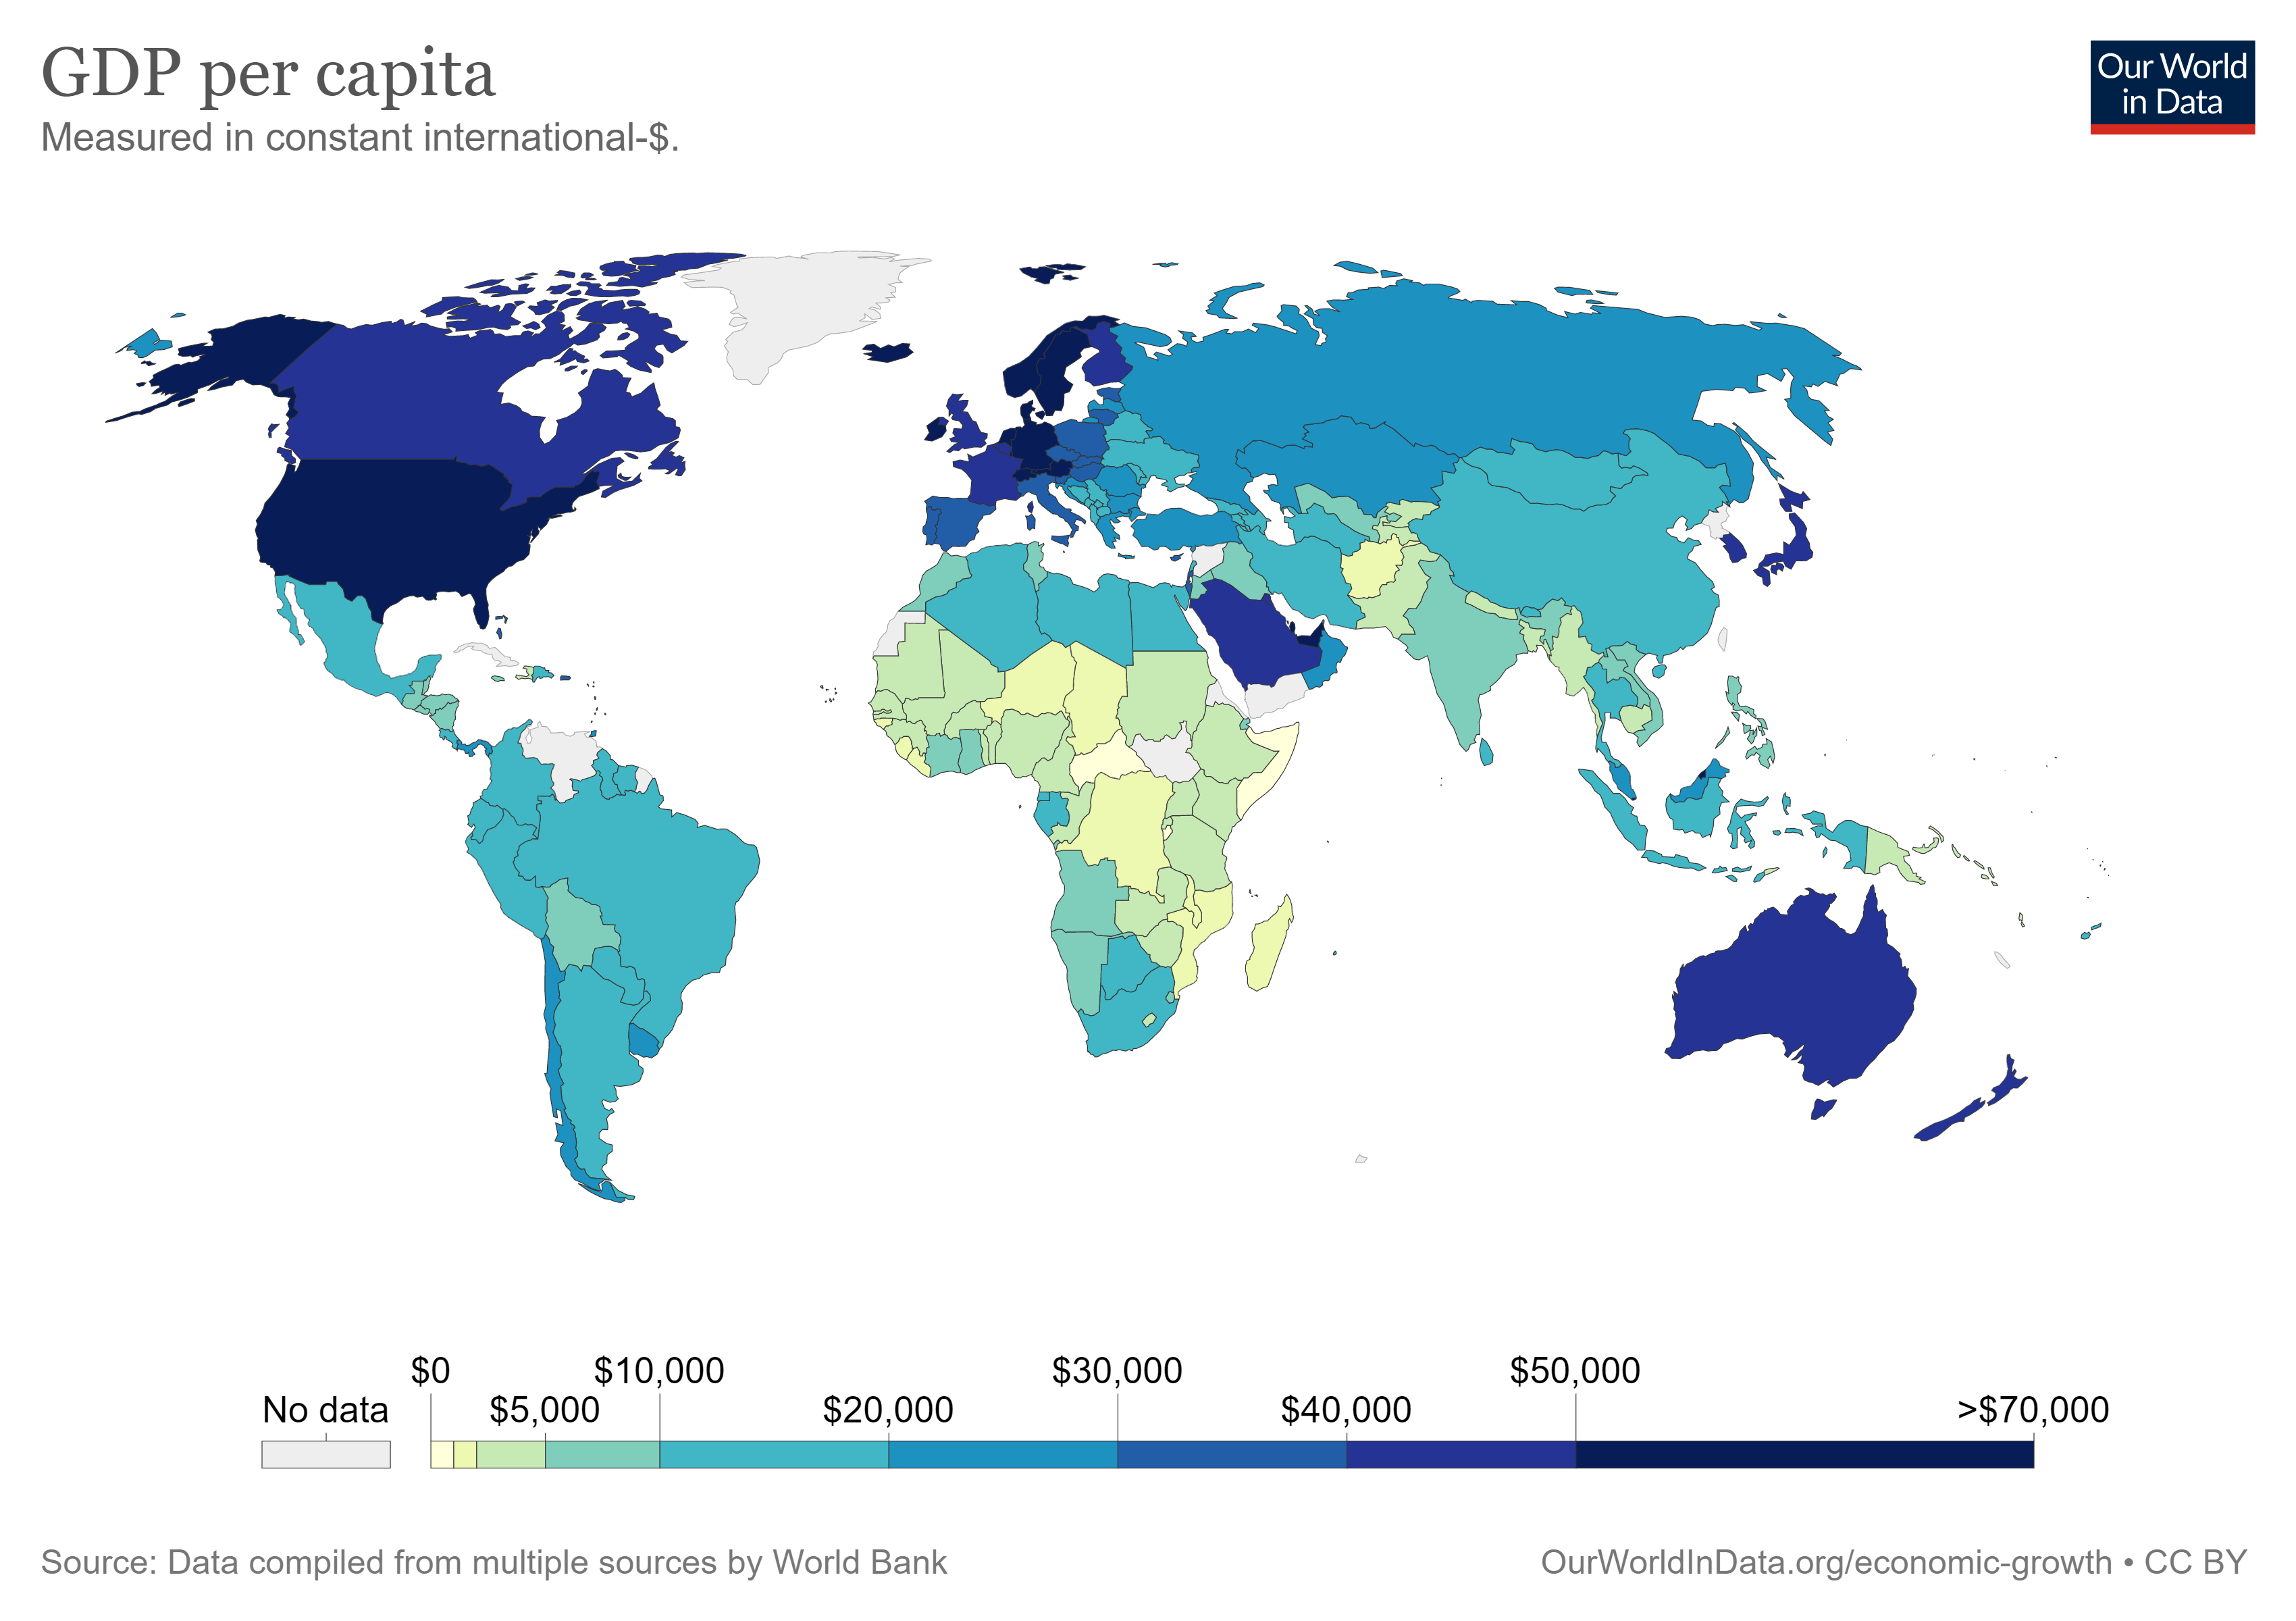
\includegraphics[width=0.9\textwidth]{Figures/gdppc2020.png}}
\end{center}
Fuente: Our World in Data
\end{frame}

\begin{frame}{Crecimiento del GDP per cápita}
    \begin{figure} [H]   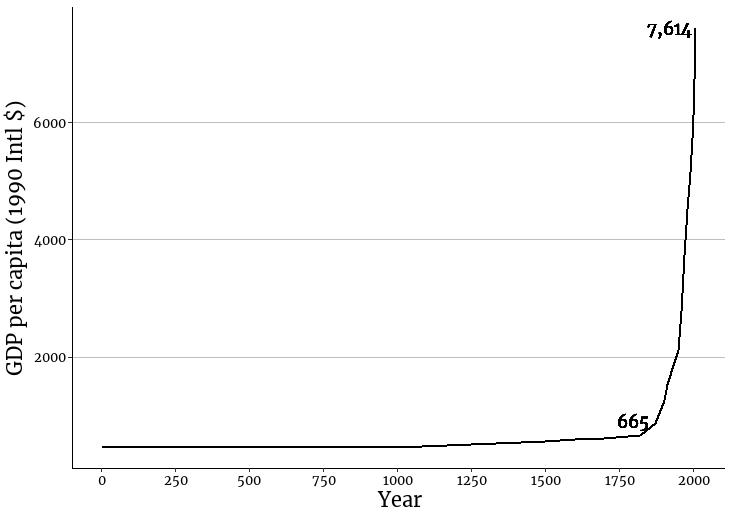
\includegraphics[scale=0.5]{Figures/C17.1.png}
\end{figure}
\end{frame}

\begin{frame}{¿Qué generó el crecimiento explosivo?}
    \begin{itemize}
    \item \textbf{Revolución industrial (desde mediados del Siglo XVIII)}
    \begin{itemize}
        \item La máquina a vapor generó una potencialidad de expansión en la producción junto con los ferrocarriles y la industria textil produjeron un aumento en el nivel de vida sin precedentes
    \end{itemize}
    
    \item \textbf{Revolución francesa (1789)}
    \begin{itemize}
        \item Permitió la movilidad social
        \item Se pasó de una sociedad estamental a una sociedad libre: mayor libertad para elegir los trabajos y ocupaciones según sus preferencias y capacidades
    \end{itemize}
     \item \textbf{Constitución de EEUU (1787)}
     \begin{itemize}
        \item Fuerte contraste con el poder absolutista de los monarcas europeos
        \item Fuertes restricciones al Estado y lo que éste podía hacer
        \item La emergencia de los gobiernos republicanos con división de poderes implicó un cambio radical en la calidad de la gestión de los recursos públicos
    \end{itemize}
\end{itemize}
\end{frame}

\begin{frame}{Felicidad y nivel de ingreso}
    \begin{figure} [H]   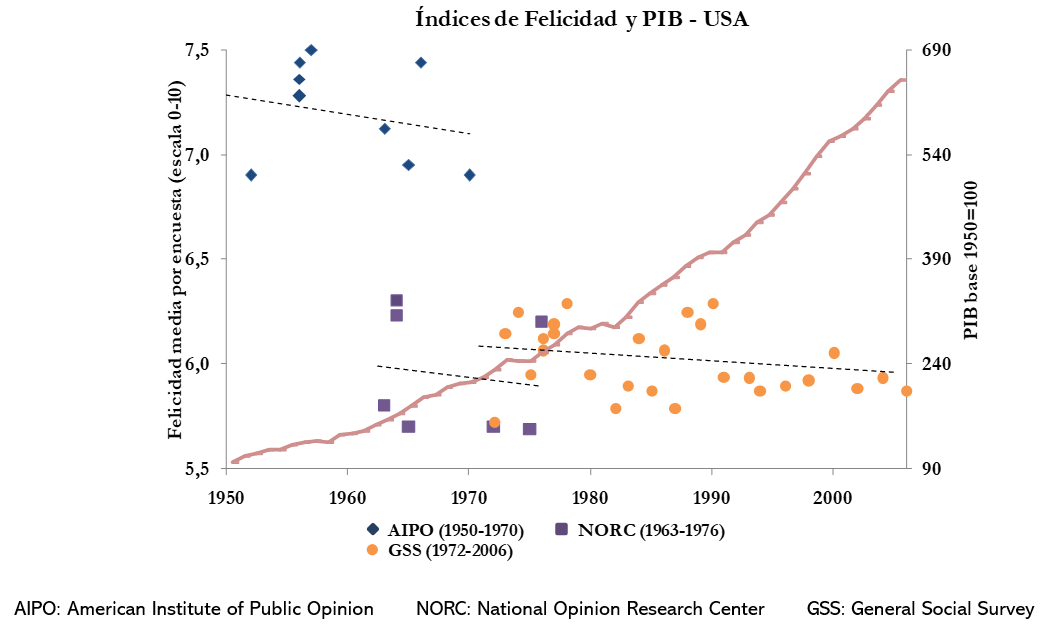
\includegraphics[scale=0.5]{Figures/C17.2.png}
\end{figure}
\end{frame}

\begin{frame}
\frametitle{Idea más amplia de bienestar}
\begin{itemize}
    \item Enfoque de capacidades de Amartya Sen
    \begin{itemize}
        \item No es lo que una persona tiene, sino lo que ella es y puede hacer \\
        - Capacidades para alcanzar su potencial como ser humano
        \item ¿Disparidad entre los ingresos y las ventajas reales? \\
        - Heterogeneidades personales, diversidad ambiental, diferencias en el clima social, distribución de recursos dentro de la familia, etc.
    \end{itemize}
    \item Índice de Desarrollo Humano (HDI) del PNUD
    \begin{itemize}
        \item Ingresos (PBI per cápita ajustado por PPP)
        \item Longevidad (esperanza de vida al nacer)
        \item Conocimiento (alfabetización y años de estudio0
    \end{itemize}
    \end{itemize}
\end{frame}

\begin{frame}
\frametitle{1HDI (2017)}
\begin{center}
    \href{https://ourworldindata.org/grapher/human-development-index?country=~ZWE} {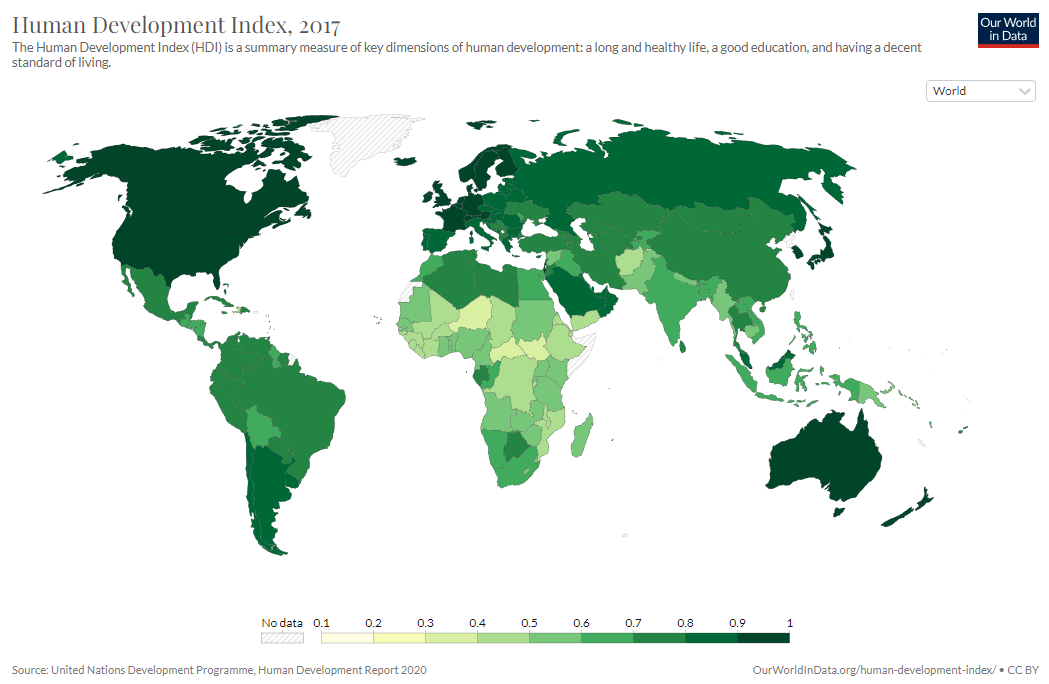
\includegraphics[scale=0.35]{Figures/Tema_11.27_hdi_PBI.png}}
\end{center}
Fuente: Our World in Data
\end{frame}

\begin{frame}
\frametitle{ PBI y desarrollo}
\begin{center}
    \href{https://ourworldindata.org/grapher/hdi-vs-gdp-per-capita} {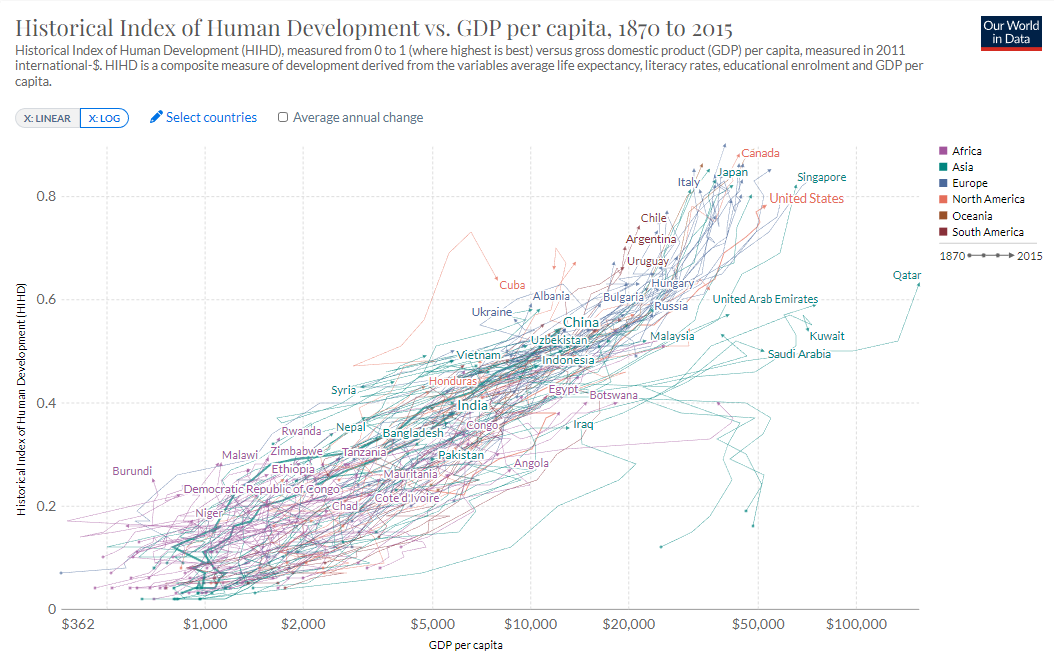
\includegraphics[scale=0.35]{Tema_11.27_hdi_2.png}}
\end{center}
Fuente: Our World in Data
\end{frame}

\begin{frame}{ La aceleración del crecimiento en gráficos}
    \begin{figure}[htp]
\href{https://www.gapminder.org/tools/} {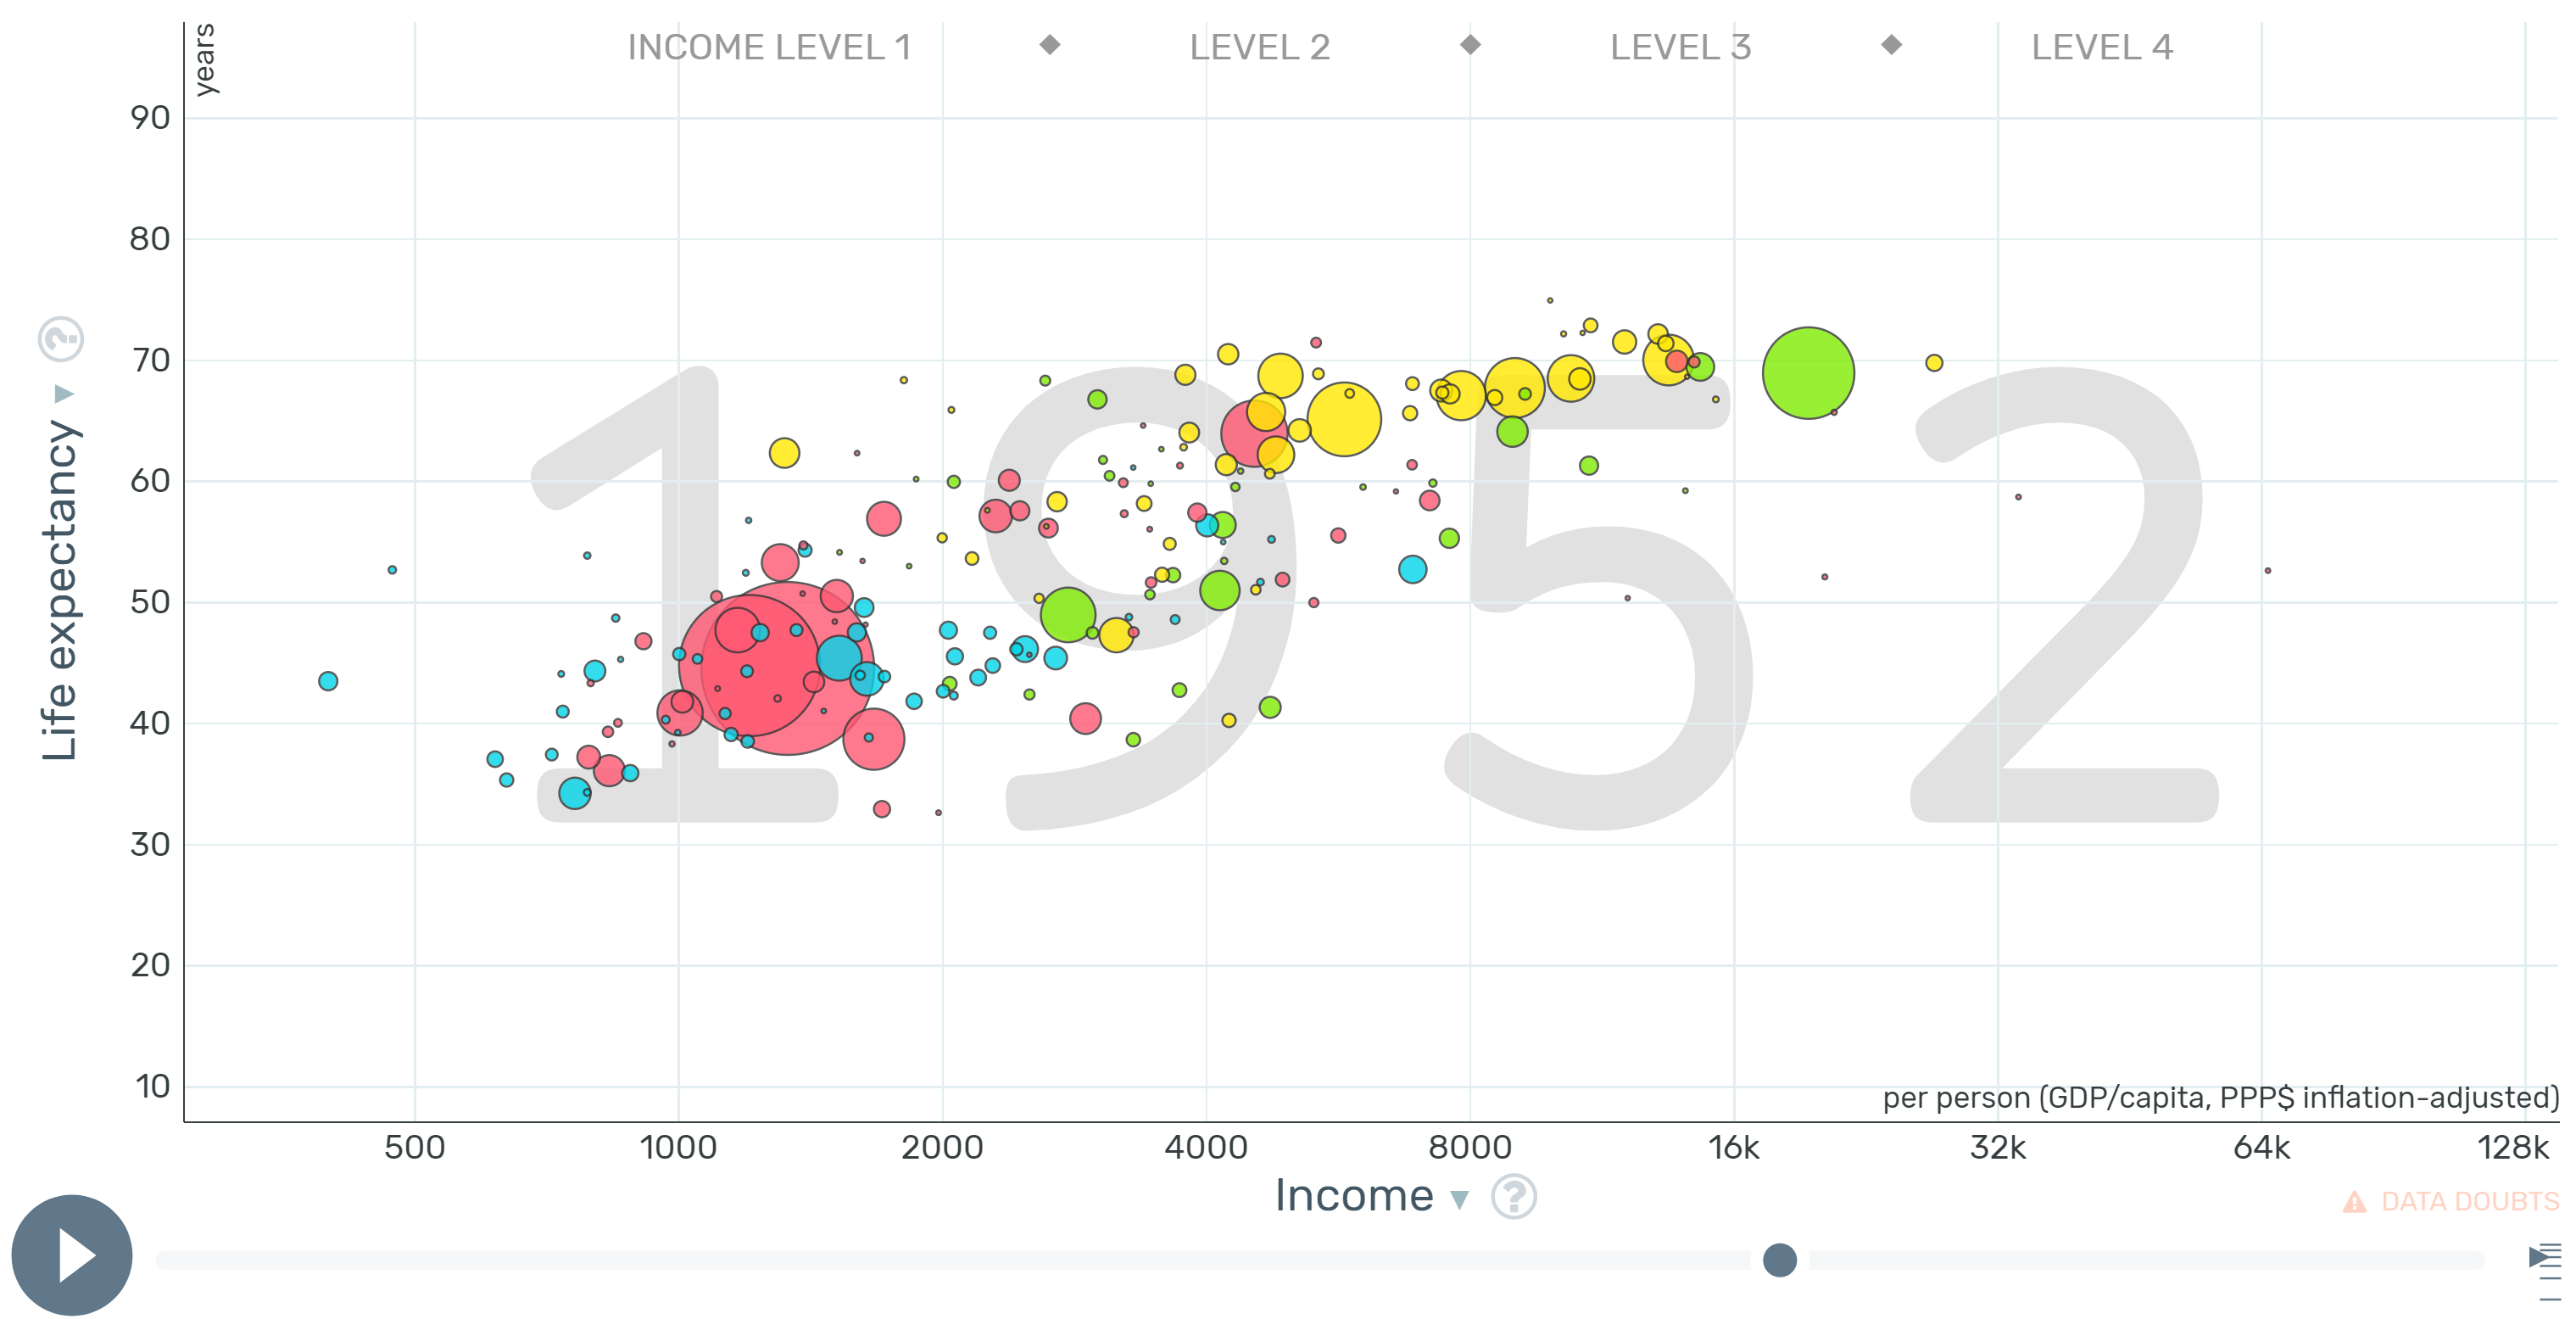
\includegraphics[width=0.99\textwidth]{Figures/Gapminder.png}} 
\end{figure}
\end{frame}

\begin{frame}{Fuentes del crecimiento}
   \begin{equation}
    Y = AF(K,L,H,RN),
\end{equation} 
\begin{itemize}
    \item El crecimiento viene de la acumulacion de factores o de la tecnologia?
    \item El hallazgo de Solow
    \item Hong Kong vs Singapur
\end{itemize}
\end{frame}

\begin{frame}{Un ejemplo de productividad}
    \begin{figure} [H]   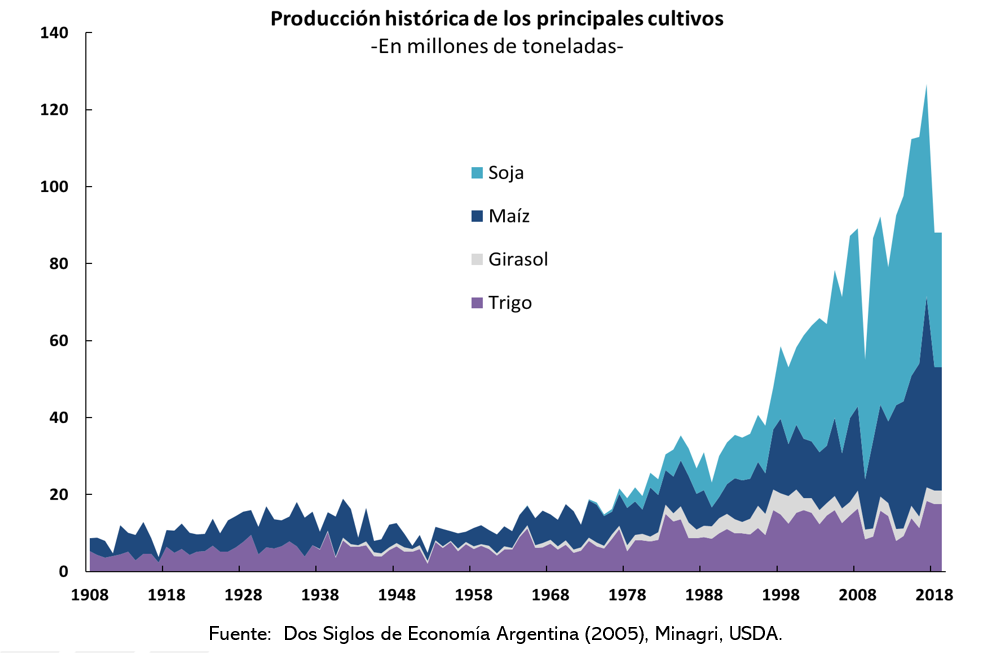
\includegraphics[scale=0.55]{Figures/C17.3.png}
\label{fig:17.3}
\end{figure}
\end{frame}


\begin{frame}{La descomposición de crecimiento para Argentina}
    \begin{figure} [H]   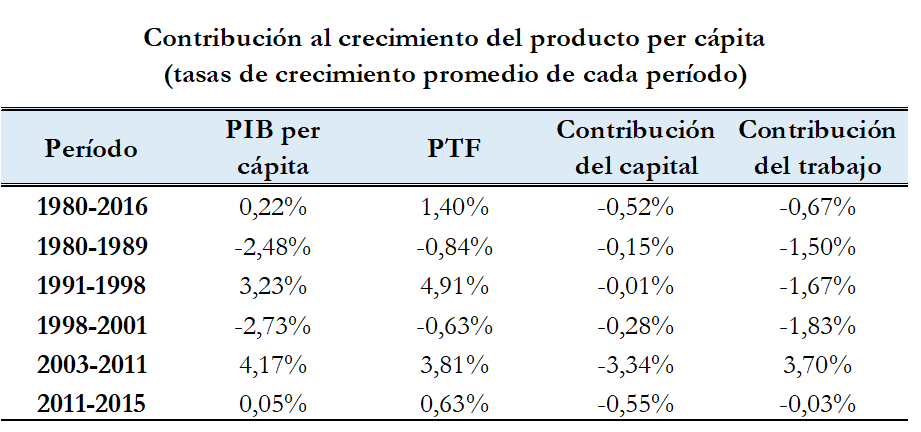
\includegraphics[scale=0.55]{Figures/C17.4.png}
\caption{\textbf{Descomposición del crecimiento de Argentina}}
\label{fig:26.4}
\end{figure}
\end{frame}


\begin{frame}{Instituciones}
    
\begin{figure}[H]
\begin{center}
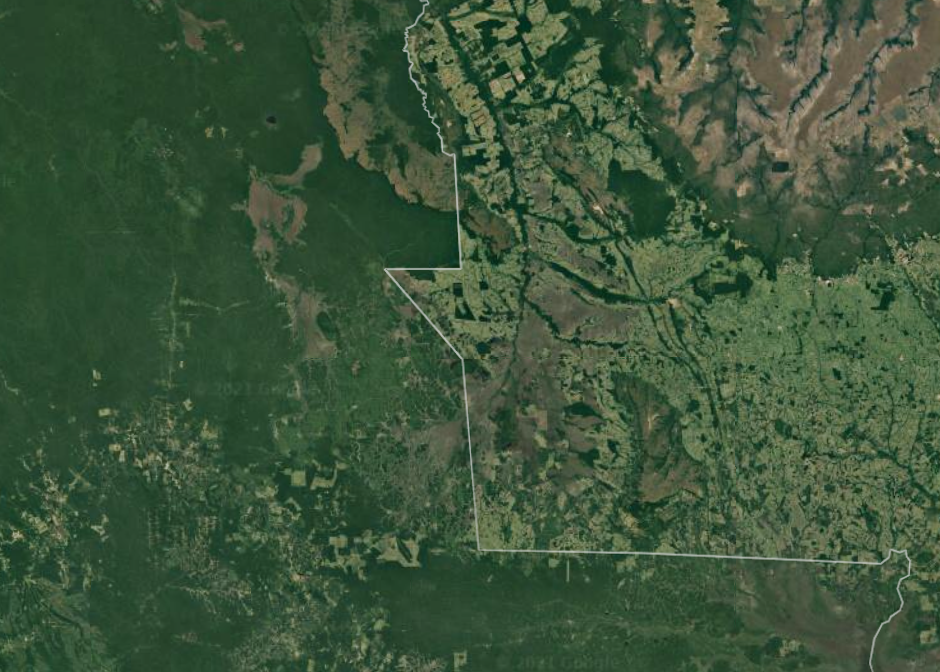
\includegraphics[width=0.8\textwidth]{Figures/C26.2.png}
\end{center}
\caption{\textbf{Frontera entre Bolivia (izquierda) y Brazil}}
\label{fig:border_bol_bra}
\end{figure}
\end{frame}

\begin{frame}{Instituciones}
    \begin{figure}[H]
\begin{center}
\includegraphics[width=0.8\textwidth]{Figures/C26.3.png}
\end{center}
\caption{\textbf{Península de Corea de noche}}
\label{fig:korea}
\end{figure}

\end{frame}


\begin{frame} 
\frametitle{ Criterios para evaluar una asignación}
\begin{itemize}
\item Hay dos criterios para evaluar una asignación específica: 
\begin{itemize}
    \item Eficiencia
    \item Equidad
\end{itemize}
\item ¿Existe un trade off entre eficiencia y equidad? No debería...
\end{itemize}
\end{frame}


\begin{frame} 
\frametitle{La desigualdad del Ingreso}
\begin{itemize}
\item Hay algunos factores importantes que determinan si una asignación es muy desigual: \begin{itemize}
    \item Diferencias en el poder de negociación.
    \item Diferencias en sus dotaciones.
    \item Instituciones.
\end{itemize}
\item Para evaluar la desigualdad, los economistas a menudo usan unas medidas llamadas Coeficiente de Gini y Curva de Lorenz.
\end{itemize}
\end{frame}

\begin{frame} 
\frametitle{El Coeficiente de Gini}
\begin{itemize}
\item El coeficiente de Gini se basa en las diferencias en los ingresos, la riqueza o alguna otra medida entre las personas. 
\item El coeficiente de Gini tiene la ventaja de que incluye información sobre todos, no solo los ricos y los pobres, sino también aquellos ``en el medio''.
\item Se calcula a partir de dos datos:
        \begin{itemize}
            \item El promedio de las diferencias entre las personas.
            \item El ingreso promedio de las personas.
        \end{itemize}
\end{itemize}
\end{frame}

\begin{frame} 
\frametitle{El Coeficiente de Gini}
\begin{itemize}
\item Coeficiente Gini = $0,5$ x  $\frac{\text{Diferencia}  \text{Promedio}}{\text{Ingreso} \text{Promedio}}$
\item En la práctica, cuando calculamos el coeficiente de Gini, obtenemos un número entre 0 (igualdad perfecta) y 1 (desigualdad extrema). 
\item Cuanto más desigualmente se distribuyen los recursos entre los miembros de la población, mayor es el coeficiente de Gini.
\end{itemize}
\end{frame}


\begin{frame} 
\frametitle{Un ejemplo}
Los círculos son personas y los números dentro de los círculos son los ingresos recibidos. Los números al lado de las flechas son las diferencias entre las dos personas, indicadas por las flechas.
    \begin{center}    
    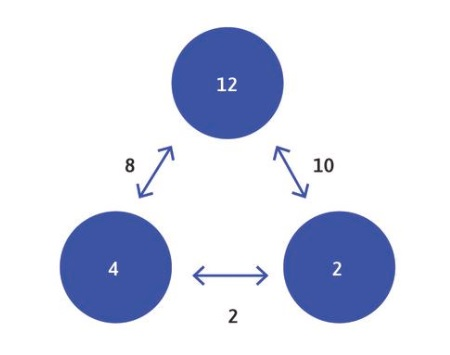
\includegraphics[scale=0.6]{Tema_04.15_gini.jpg}
    \end{center}
\end{frame}

\begin{frame} 
\frametitle{Un ejemplo}
\begin{itemize}
    \item El promedio de las diferencias entre las personas es \\ (10 + 8 + 2) / 3 = 20/3 = 6,67 \\ \vspace{3mm}
    \item El ingreso promedio de las personas es \\ (12 + 4 + 2) / 3 = 6.
\end{itemize}
\vspace{3mm}

El coeficiente de Gini es igual a 0,5,(6,67/6) = 0,56
\end{frame}

\begin{frame} 
\frametitle{La curva de Lorenz}
\begin{itemize}
\item Es una herramienta útil para observar la distribución completa del ingreso o la riqueza que representa y comparar las distribuciones del ingreso o la riqueza entre los países.  
\item Es una representación gráfica de la desigualdad de cierta cantidad, como la riqueza o el ingreso.
\item Indica cuánta disparidad hay en el ingreso, o en cualquier otra medida, a través de la población.
\end{itemize}
\end{frame}

\begin{frame} 
\frametitle{La curva de Lorenz}
\begin{itemize}
\item Los individuos se organizan en orden ascendente según el ingreso que tienen, y la parte acumulada del ingreso se grafica contra la parte acumulada de la población.
\item Para la igualdad completa de ingresos, la curva de Lorenz sería una línea recta con una pendiente igual a uno.
\item La medida en que la curva cae por debajo de esta línea de igualdad perfecta es una medida de la desigualdad.
\end{itemize}
\end{frame}

\begin{frame}{La distribución del ingreso la curva de Lorenz}
    \begin{figure} [H]
\centering
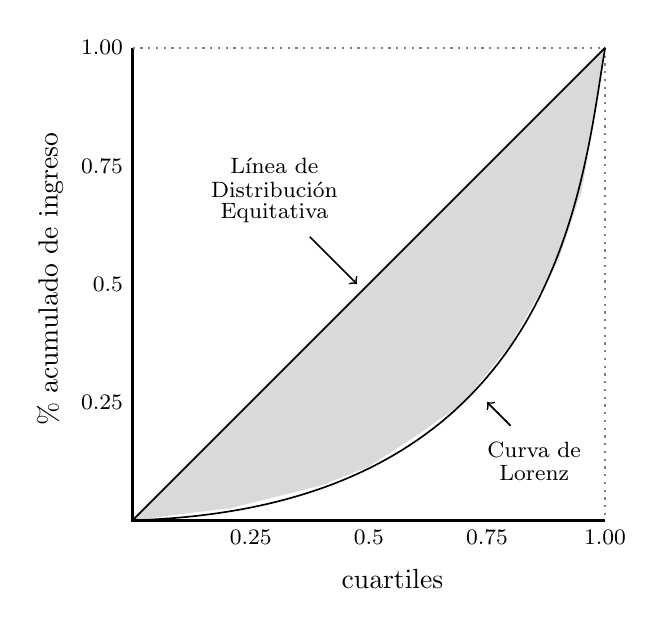
\begin{tikzpicture}[scale=0.6]
\draw[fill,gray!30] (0,0)--(10,10)--(9.5,7)--(9,5.5)--(8,3.75)--(7,2.5)--(6,1.8)--(5,1.15)--(4,0.75)--(2,0.25);
\draw[very thick,-] (0,10) node[above]{}--(0,0)--(10,0) node[right]{};
\draw[thick, dotted, gray] (0,10)--(10,10)--(10,0);
\draw[semithick] (0,0)--(10,10);
\draw[semithick] (0,0)..controls (9,0.25) and (9.5,7)..(10,10);
\node at (-1.75, 5){\rotatebox{90}{ \% acumulado de ingreso}};
\node[] at (5.5,-1.25) { cuartiles};
\node[below] at (2.5,0){\footnotesize 0.25};
\node[below] at (5,0){\footnotesize 0.5};
\node[below] at (7.5,0){\footnotesize 0.75};
\node[below] at (10,0){\footnotesize 1.00};
\node[left] at (0,2.5){\footnotesize 0.25};
\node[left] at (0,5){\footnotesize 0.5};
\node[left] at (0,7.5){\footnotesize 0.75};
\node[left] at (0,10){\footnotesize 1.00};
\node[] at (3,7.5) {\footnotesize Línea de };
\node[] at (3,7) {\footnotesize Distribución};
\node[] at (3,6.5) {\footnotesize Equitativa };
\draw[semithick, ->] (3.75,6)--(4.75,5);
\node[] at (8.5,1.5) {\footnotesize Curva de };
\node[] at (8.5,1) {\footnotesize Lorenz };
\draw[semithick, ->] (8,2)--(7.5,2.5);
\end{tikzpicture}
\end{figure} 
\end{frame}

%\begin{frame} 
%\frametitle{Un ejemplo aplicado}
%    \begin{center}    
%    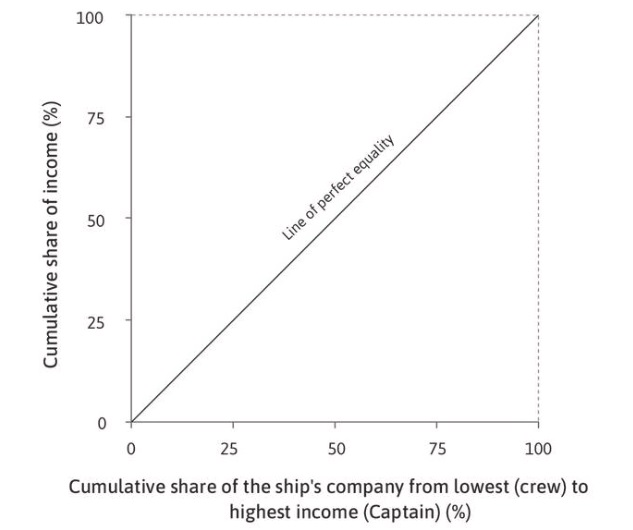
\includegraphics[scale=0.55]{Tema_04.16_lorenz1.jpg}
%    \end{center}
%\end{frame}
%\begin{frame} 
%\frametitle{Un ejemplo aplicado}
%    \begin{center}    
%    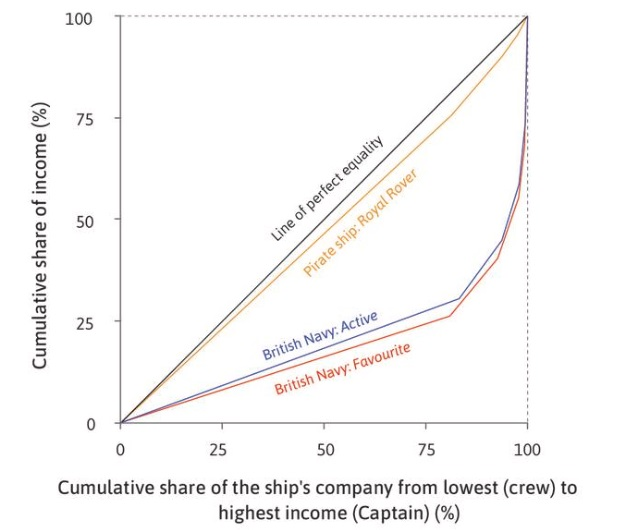
\includegraphics[scale=0.55]{Tema_04.17_lorenz2.jpg}
%    \end{center}
%\end{frame}

\begin{frame} 
\frametitle{El coeficiente de Gini y la curva de Lorenz}
\begin{itemize}
\item Existe una relación muy simple entre la curva de Lorenz y el coeficiente de Gini. 
\item Puede ver que las distribuciones más desiguales tienen un área mayor entre la curva de Lorenz y la línea de 45 grados. 
\item El coeficiente de Gini se puede calcular como la relación entre esta área y el área de todo el triángulo debajo de la línea de 45 grados.
\end{itemize}
\end{frame}

\begin{frame}{El coeficiente de Gini}
    \begin{figure} [H]
\centering
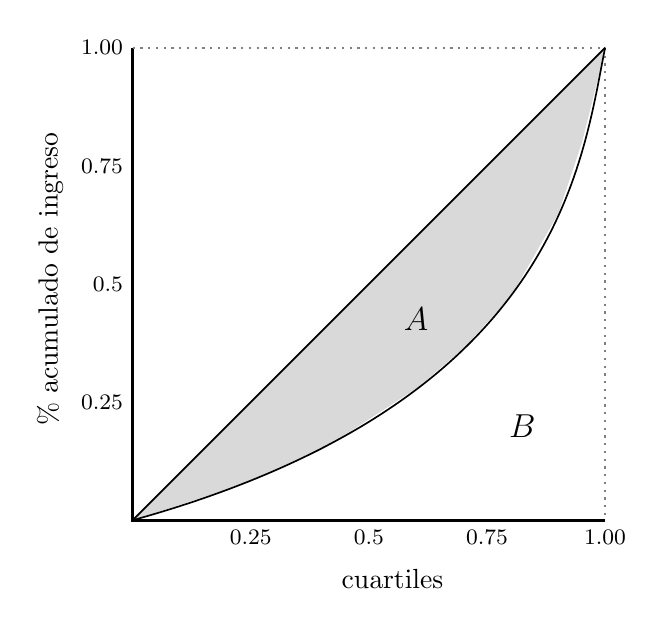
\begin{tikzpicture}[scale=0.6]
\draw[fill,gray!30] (0,0)--(10,10)--(9.5,8)--(9,6.5)--(8,4.75)--(7,3.65)--(6,2.8)--(5,2.15)--(4,1.5)--(2,0.65);
\draw[very thick,-] (0,10) node[above]{}--(0,0)--(10,0) node[right]{};
\draw[thick, dotted, gray] (0,10)--(10,10)--(10,0);
\draw[semithick] (0,0)--(10,10);
\draw[semithick] (0,0)..controls (9,2.5) and (9.5,7.5)..(10,10);
\node at (-1.75, 5){\rotatebox{90}{ \% acumulado de ingreso}};
\node[] at (5.5,-1.25) { cuartiles};
\node[below] at (2.5,0){\footnotesize 0.25};
\node[below] at (5,0){\footnotesize 0.5};
\node[below] at (7.5,0){\footnotesize 0.75};
\node[below] at (10,0){\footnotesize 1.00};
\node[left] at (0,2.5){\footnotesize 0.25};
\node[left] at (0,5){\footnotesize 0.5};
\node[left] at (0,7.5){\footnotesize 0.75};
\node[left] at (0,10){\footnotesize 1.00};
\node[] at (6,4.25) {\large $A$};
\node[] at (8.25,2) {\large $B$};
\end{tikzpicture}
\end{figure} 
\end{frame}



\begin{frame} 
\frametitle{El coeficiente de Gini y la curva de Lorenz}
\begin{itemize}
\item Si todos tienen el mismo ingreso (no hay desigualdad de ingresos), el coeficiente de Gini toma un valor de 0. Esto se debe a que la curva de Lorenz sería exactamente la línea de la igualdad perfecta, por lo que no habría área entre los dos.
\item $G=\frac{A}{A+B}$
\item Este método de cálculo del Gini solo da una aproximación. La aproximación del área sólo es precisa cuando la población es grande.
\end{itemize}
\end{frame}

\begin{frame} 
\frametitle{Un ejemplo aplicado}
    \begin{center}    
    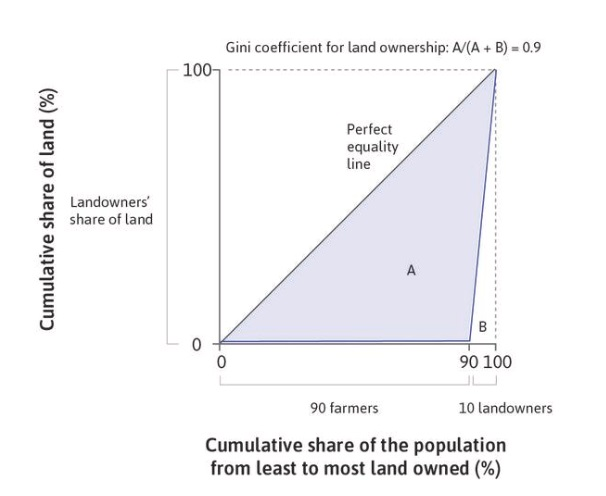
\includegraphics[scale=0.55]{Tema_04.18_lorenz3.jpg}
    \end{center}
\end{frame}

\begin{frame} 
\frametitle{ Un ejemplo aplicado}
    \begin{center}    
    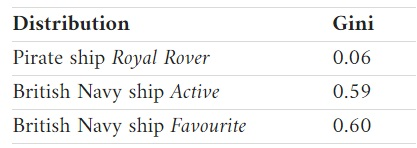
\includegraphics[scale=0.75]{Tema_04.19_gini2.jpg}
    \end{center}
\end{frame}

\begin{frame} 
\frametitle{Diferentes variedad de desigualdad}
\begin{itemize}
\item ¡No todas las desigualdades son iguales!
\item No es lo mismo que una sociedad sea altamente desigual porque hay un pequeño número de personas excepcionalmente ricas y todos los demás están en una situación de buena posición económica o que sea desigual porque hay un pequeño número de personas muy pobres, y todos los demás están en mejores condiciones.
\end{itemize}
\end{frame}

\begin{frame} 
\frametitle{ Diferentes variedad de desigualdad}
\begin{itemize}
\item Estas dos sociedades podrían tener el mismo coeficiente de Gini, pero pensaríamos que son bastante diferentes en la naturaleza de la desigualdad que experimentan.
\end{itemize}
\end{frame}

\begin{frame} 
\frametitle{ Un ejemplo aplicado}
    \begin{center}    
    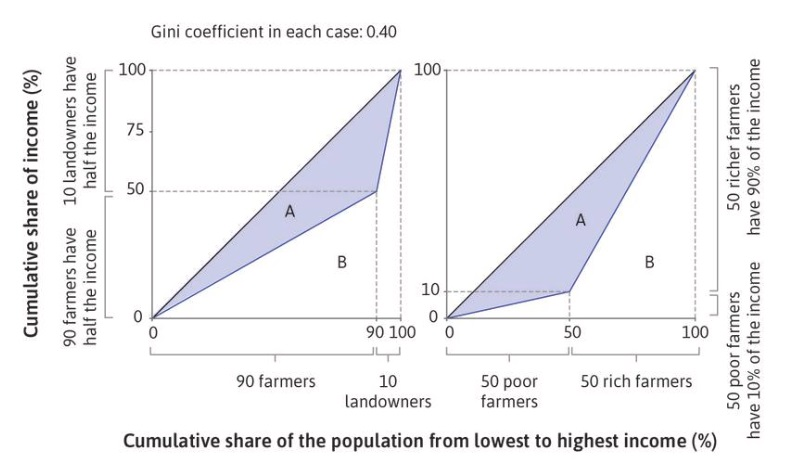
\includegraphics[scale=0.55]{Tema_04.20_variedaddesigual.jpg}
    \end{center}
\end{frame}

\begin{frame} 
\frametitle{ Diferentes variedad de desigualdad}
\begin{itemize}
\item En la figura anterior hay dos sociedad con el mismo coeficiente de Gini.
\item El área $\frac{A}{A + B}$ es la misma en cada curva de Lorenz, pero la distribución del ingreso está lejos de ser idéntica.
\item En la sociedad de la izquierda, la mitad del ingreso total se divide entre 90 agricultores mientras que 10 terratenientes obtienen la mitad restante. 
\end{itemize}
\end{frame}

\begin{frame} 
\frametitle{ Diferentes variedad de desigualdad}
\begin{itemize}
\item En la sociedad que se muestra a la derecha, 50 agricultores pobres obtienen una décima parte de los ingresos para dividirse entre ellos y 50 agricultores más ricos dividen el 90\% restante.
\end{itemize}
\end{frame}

\begin{frame}{Evolución de la pobreza en el mundo}
    \begin{figure} [H]
    \centering
     \href{https://www.gapminder.org/tools/#$model$markers$bubble$encoding$frame$speed:139;;;;;&chart-type=bubbles&url=v1}{
    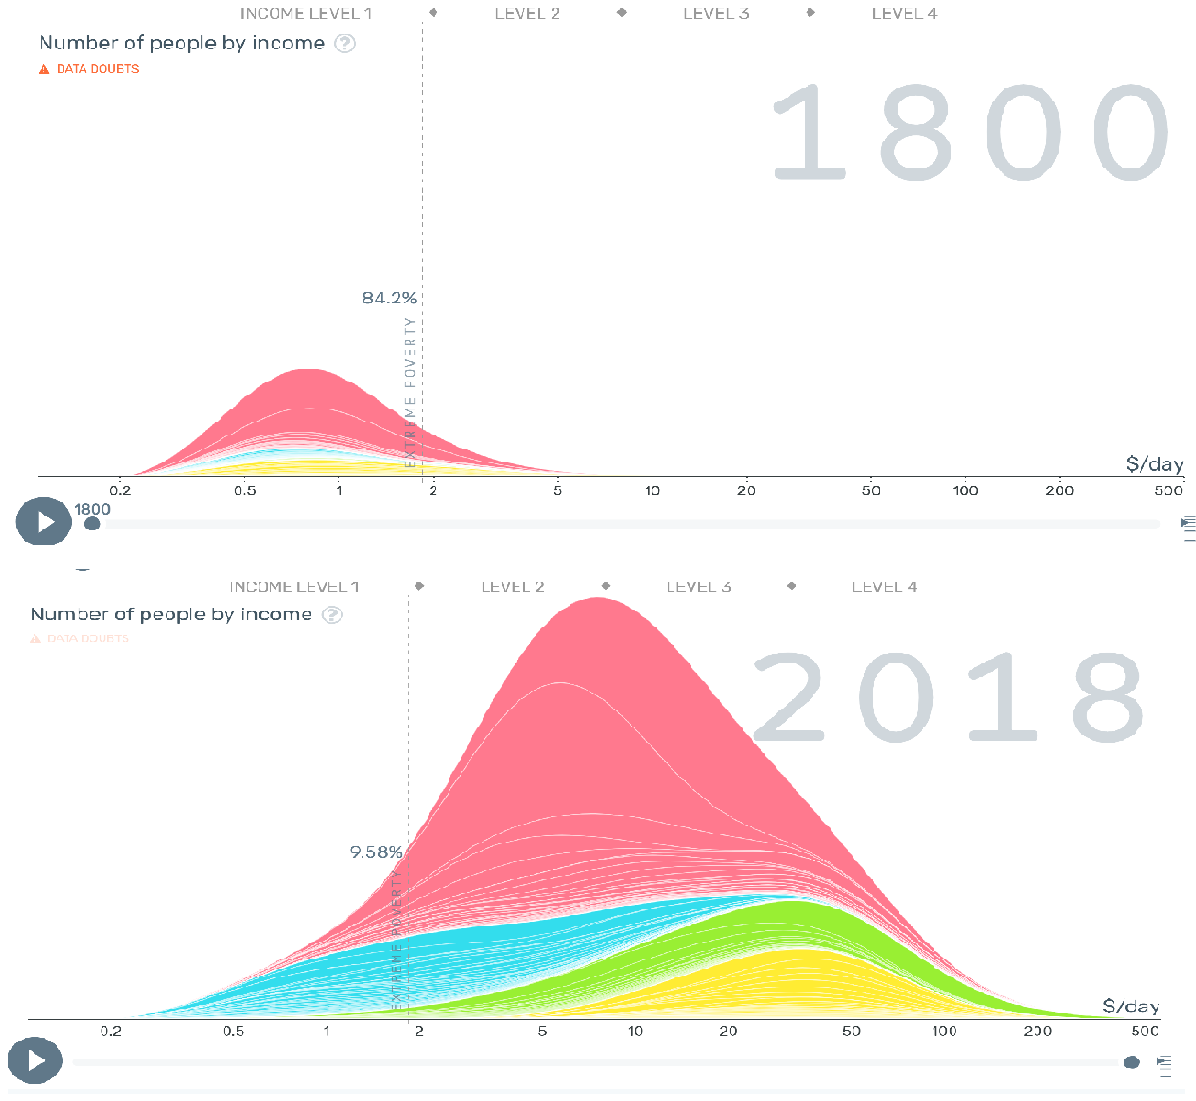
\includegraphics[scale=0.75]{Figures/Gapminder3.png}}
\end{figure}
\end{frame}


\begin{frame}{Discusión}
\begin{itemize}
    \item The college premium
    \item Distribución del ingreso global vs cada país
    \item El debate de Piketty
    \item El concepto de justicia de Rawls 
\end{itemize}
    
\end{frame}

\begin{frame}{ El ciclo económico}
    \begin{figure} [H]   
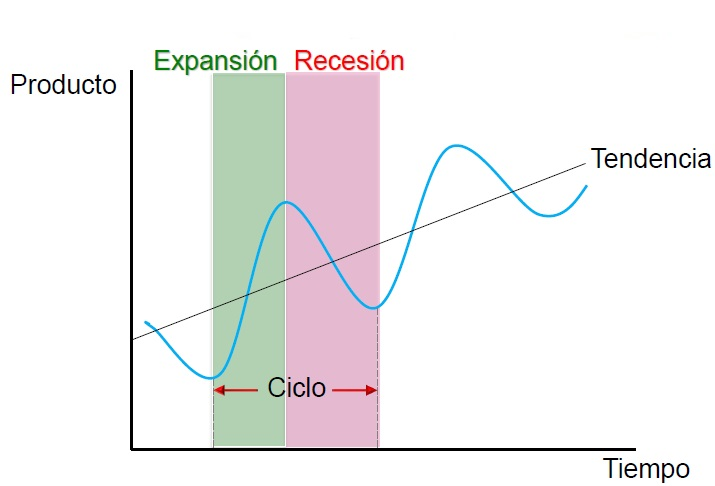
\includegraphics[scale=0.55]{Figures/C19.1.jpg}
\label{fig:19.1}
\end{figure}
\end{frame}

\begin{frame}
\frametitle{Nivel y tasa de crecimiento del PBI }
\begin{itemize}
    \item El PBI nos da una medida de la magnitud de la economía, pero es su tasa de cambio la que nos dice cómo la economía está evolucionando \\ \vspace{2mm}
    Tasa de cambio = $\frac{PBI_t-PBI_{t-1}}{PBI_{t-1}}=\frac{\Delta PBI_{t}}{PBI_{t-1}} $
    \vspace{2mm}
    \begin{itemize}
        \item Normalmente se llama recesión al (los) período(s) en el cuál esta tasa es negativa durante tres trimestres consecutivos
        \item Los períodos de crecimiento del PBI son expansiones
    \end{itemize}
\end{itemize}
\end{frame}

\begin{frame}{Crecimiento del PBI de Argentina (\% anual)}
    \begin{figure}[htp]
\href{https://datos.bancomundial.org/share/widget?indicators=NY.GDP.MKTP.KD.ZG&locations=AR" width='450' height='300' frameBorder='0' scrolling="no"} {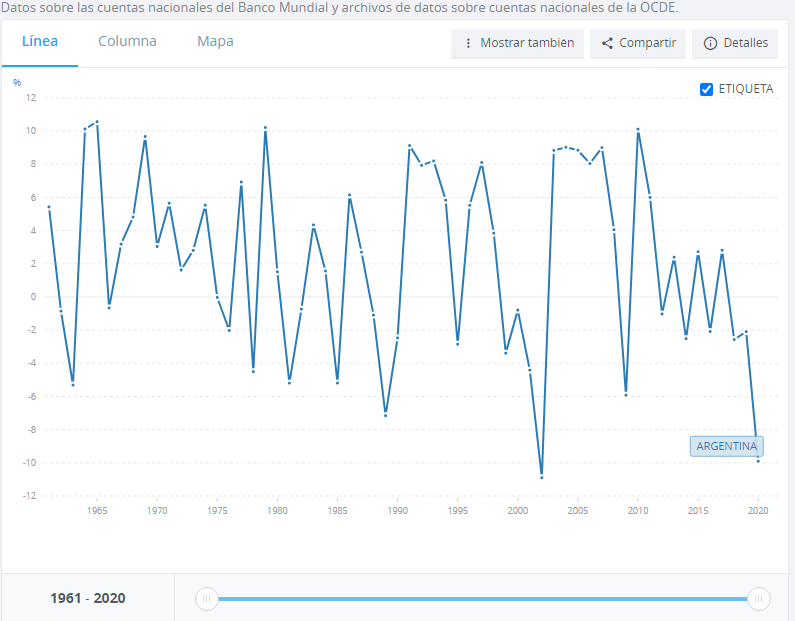
\includegraphics[width=0.90\textwidth]{Figures/PBIargentina.png}} 
\end{figure}
\end{frame}

\begin{frame}{Ciclos en el PBI en EEUU}

\centering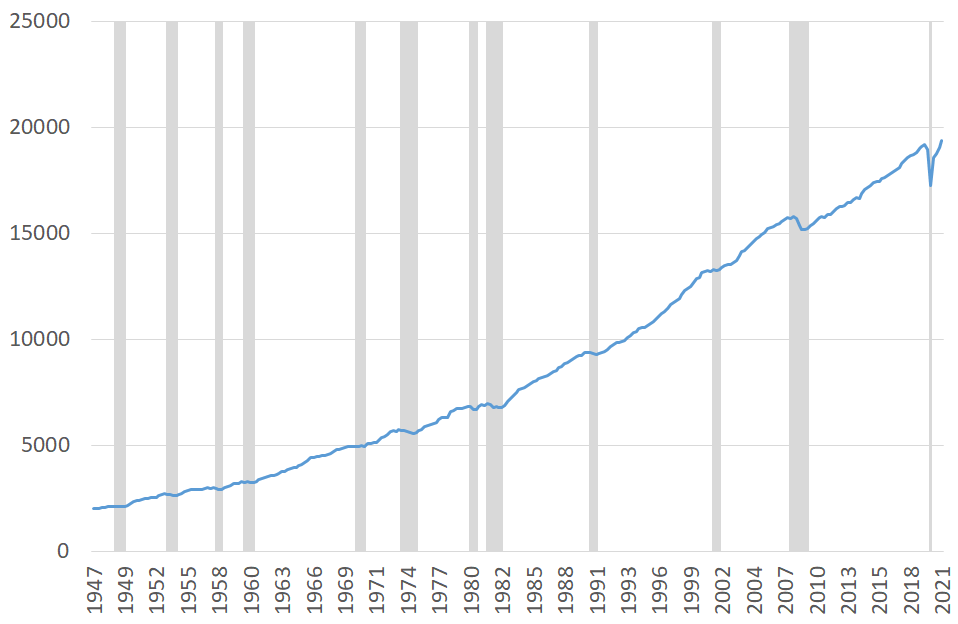
\includegraphics[width=11cm]{USA_Rec.png}\

\end{frame}


\begin{frame}{Ciclos en el PBI en Argentina}

\centering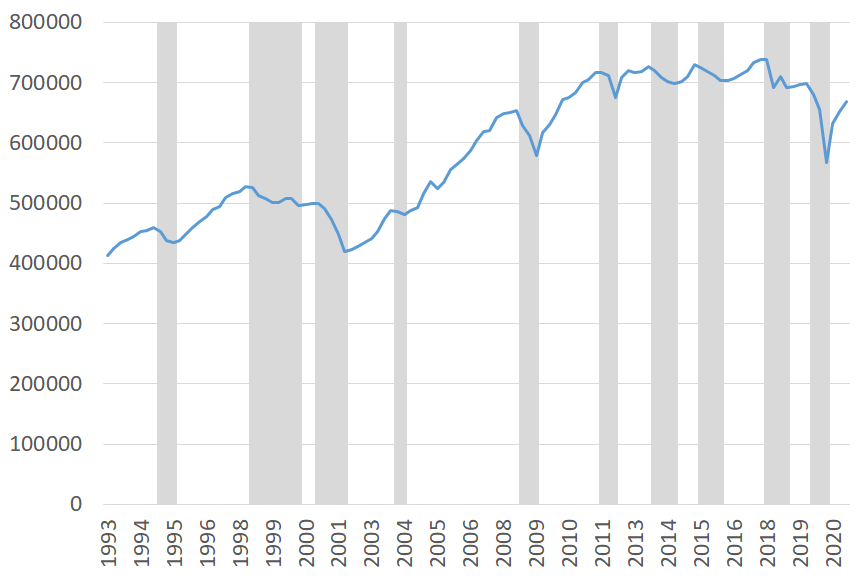
\includegraphics[width=11cm]{Figures/ARG_Rec.png}\

\end{frame}


\begin{frame}{ Estimando el ciclo}

\centering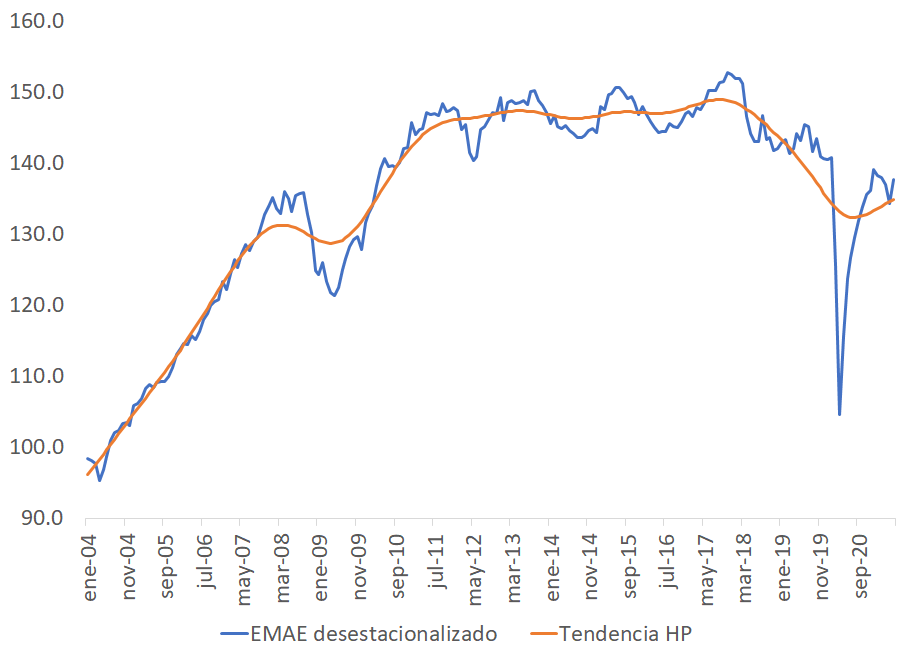
\includegraphics[width=11cm]{Figures/G9.png}\

\end{frame}


\begin{frame}{ Ciclos Económicos comparados}

\centering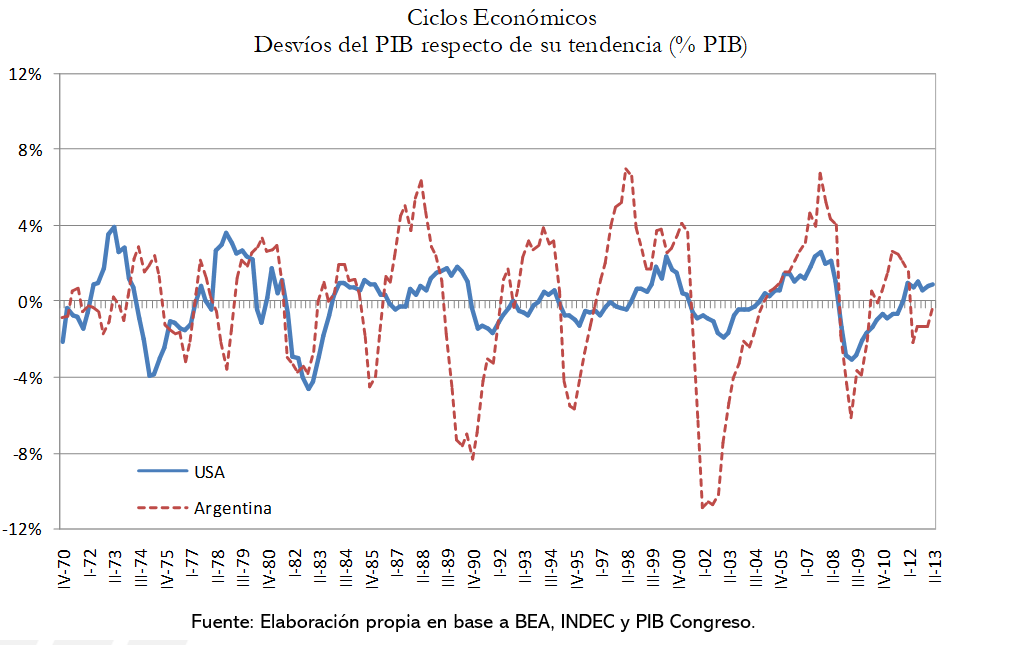
\includegraphics[width=12cm]{Figures/P12.png}\

\end{frame}


\begin{frame}{Datos con estacionalidad vs. desestacionalizados}
\centering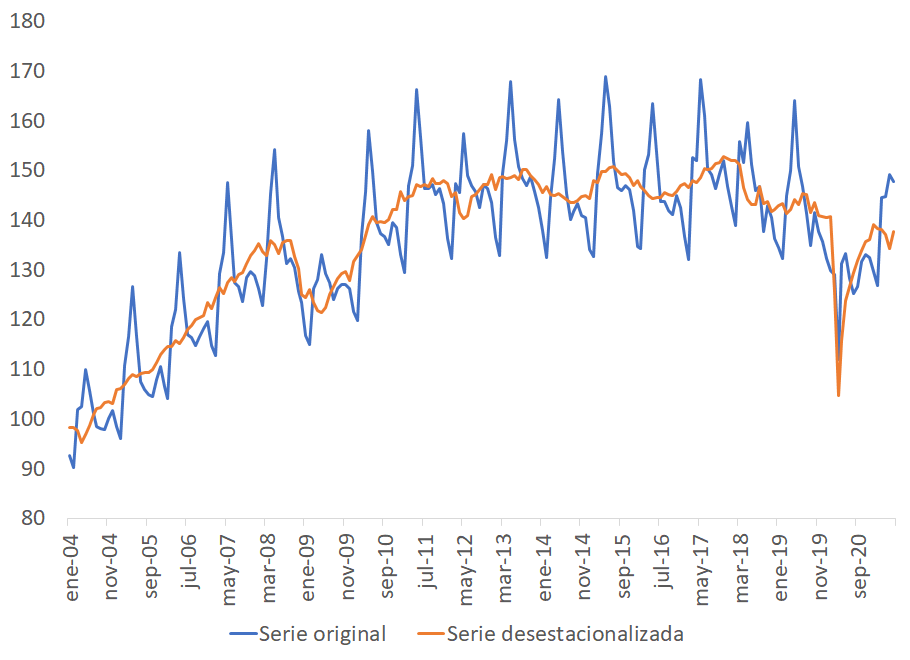
\includegraphics[width=11cm]{Figures/G11.png}\
\end{frame}


\begin{frame}{Arrastre estadístico}

\centering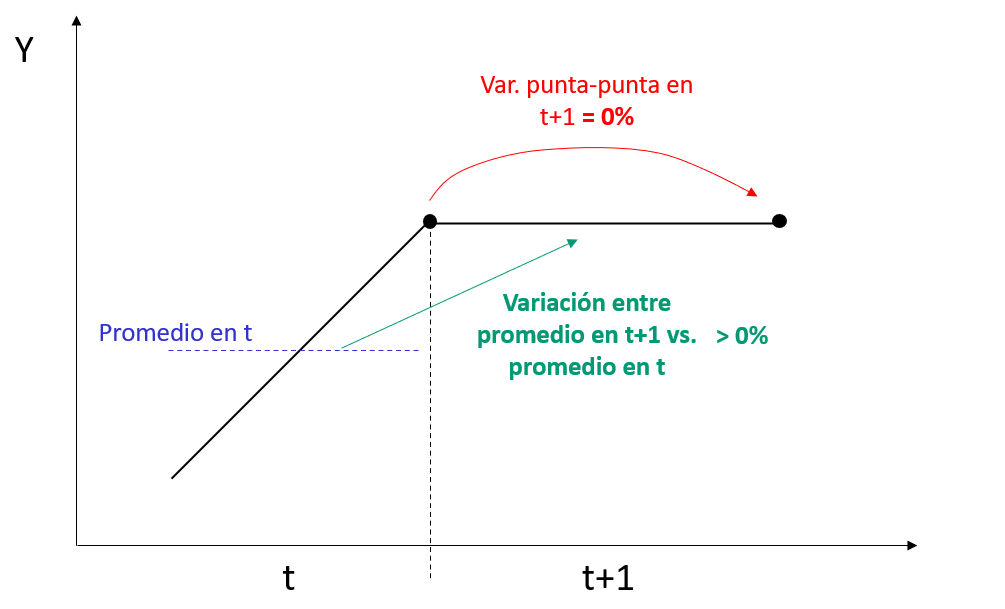
\includegraphics[width=12cm]{Figures/P11.png}\

\end{frame}


\begin{frame}{Evolución reciente del nivel de actividad}

\centering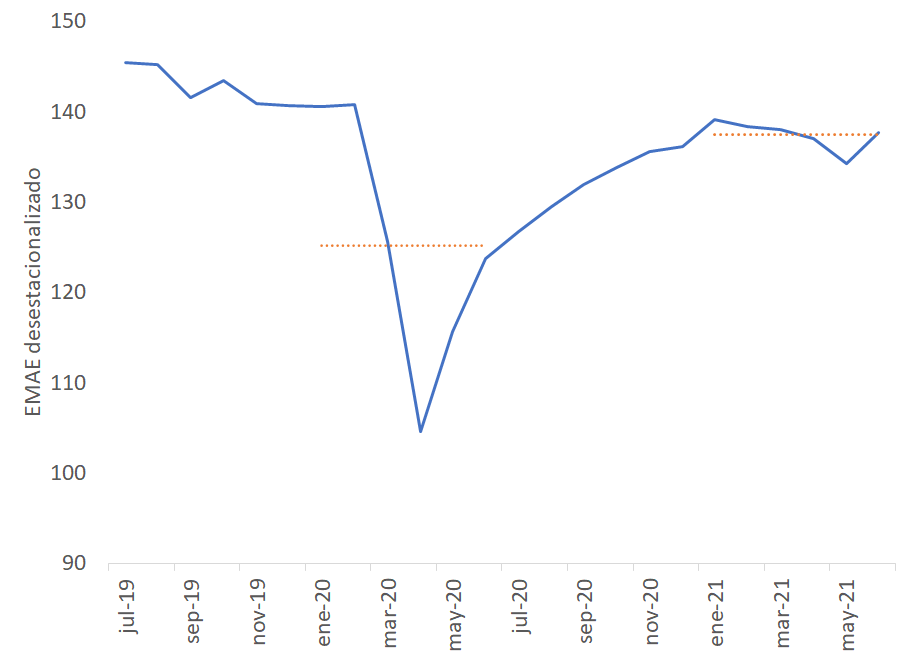
\includegraphics[width=11cm]{Figures/G12.png}\

\end{frame}


\end{document}